\chapter{Referencial teórico}\label{ch:fundamentacao}

Quando trabalhamos com um conjunto de dados relativamente grande, parte deste tende a ser distribuído entre os níveis da hierarquia de memória, 
podendo acarretar em um alto número de transferência de dados entre níveis e consequentemente numa piora do desempenho geral do sistema. 

Este capítulo discorre sobre a importância do estudo e implementação de estruturas de dados sucintas afim de sanar o problema do alto número de transferências
de dados entre diferentes níveis da memória, apresentando também conceitos básicos de representações que são amplamente usadas na construção dessas estruturas. 

\section{Avanços tecnológicos e estrutura de dados sucintas}
A divisão da indústria de microprocessadores e memória gera o que conhecemos como  gargalo de comunicação entre processador e  memória principal - gargalo de Von-Neumann - isso se deve em partes ao fato de que a indústria de processadores visa desenvolver uma lógica que acelera a comunicação, ao passo que os fabricantes de memória tem por objetivo aumentar a capacidade de armazenamento de dados \citep{paper-processor-memory-bottleneck}, esses diferentes objetivos fazem com que o desempenho desses dois componentes cresça com uma diferença de 50\%  ao ano, como ilustrado na \figref{fig:processor-memory-performance-gap}.
\begin{figure}[!ht]
\centering
  \caption[Lacuna de desempenho entre processador e memória a cada dois anos, começando de 1980]{Lacuna de desempenho entre processador e memória a cada dois anos, começando de 1980}
  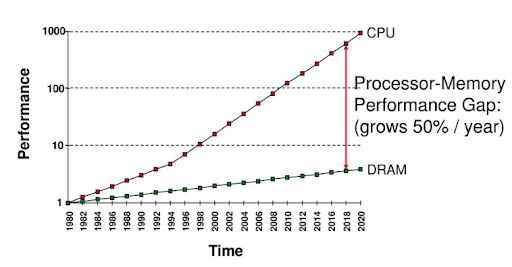
\includegraphics[scale=0.7]{images/gap-processor-memory.png}
  \footnotesize{Retirado de: http://mirkwood.cs.edinboro.edu/~bennett/class/csci312/fall2018/notes/five/one.html}
  \label{fig:processor-memory-performance-gap}
\end{figure} 

Apesar das melhorias feitas por cada uma destas indústrias ao longo dos anos, a disparidade de desempenho dos dois componentes fazem com que o processador imponha demandas significativas à memória, que em um cenário real não podem ser supridas, gerando assim um sistema desequilibrado, e então, devido a baixa largura de banda da memória em comparação ao alto desempenho do processador temos um aumento no tempo gasto para concluir uma solicitação, afetando diretamente o desempenho das aplicações.
Para suprir esse desequilíbrio os projetistas de computadores criaram o que conhecemos como hierarquia de memória, que consiste em conectar o processador 
\begin{quotation}[]
`"a um conjunto hierárquico de memórias, cada uma das quais maior, mais lenta e mais barata (por byte) do que as memórias mais próximas ao processador" \cite[tradução nossa]{paper-gap-between-processor-memory}.
\end{quotation}

Nas arquiteturas computacionais modernas essa hierarquia é formada por: registradores, cache, memória primária e memória secundária. A \figref{fig:hierarquia-de-memoria} 
demonstra uma hierarquia de memória e os seus respectivos valores de latência  e espaço para cada nível de um servidor e um dispositivo móvel hipotético. Pela figura é
possível observar que, à medida que nos distanciamos do processador, as unidades de tempo sobem à fatores de $10^9$ — de picossegundos para milissegundos — 
e as unidades de tamanho mudam por fatores de $10^{12}$ — de bytes para terabytes.

Devido  a baixa latência que as memórias mais distantes do processador possuem, torna-se ideal para obter um desempenho efetivo das operações sobre um conjunto de dados, trabalhar nos níveis superiores da hierarquia de memória \citep{book-compact-data-structures}. A grande problemática é que como vemos em \citet{paper-gap-between-processor-memory}, as memórias com latência menor possuem capacidade de armazenamento também menor, tornando praticamente inviável manipular grandes conjuntos de dados nestes níveis, o que é cada vez mais comum nos dias atuais. Uma possível solução para tanto é operar sobre os dados em sua forma compactada
e conforme cita também \citeauthor{coira-feranando}, a melhor maneira de fazer isso é através do uso das estruturas de dados sucintas.
%TODO: melhor pelo paragŕafo abaixo
\begin{figure}[!ht]
\centering
  \caption[Exemplos de representação gráficas de árvores]{Os níveis em uma hierarquia de memória em um servidor (a) e em um dispositivo pessoal móvel (PMD) (b).}
  \subfigure[ref1][Hierarquia de memória de um servidor]{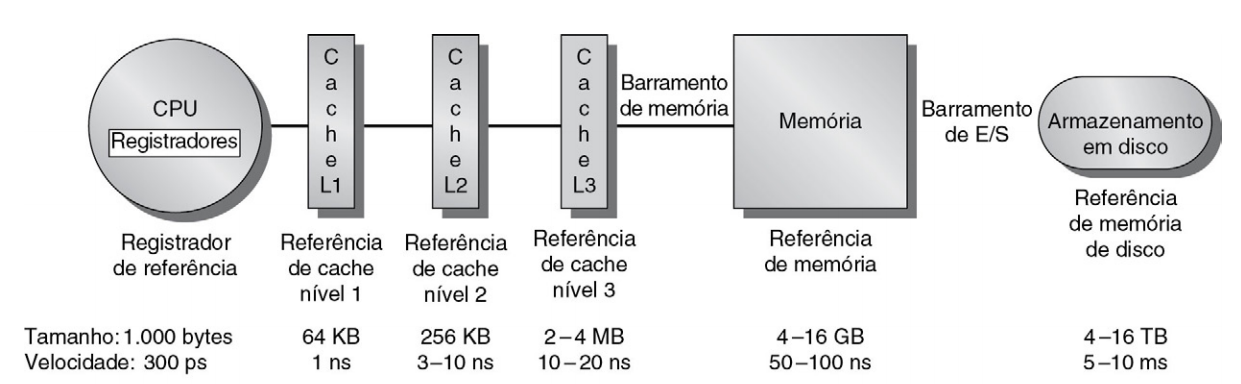
\includegraphics[width=\columnwidth]{images/servidor.png}}
  \qquad
  \subfigure[ref1][Hierarquia de memória de um dispositivo móvel]{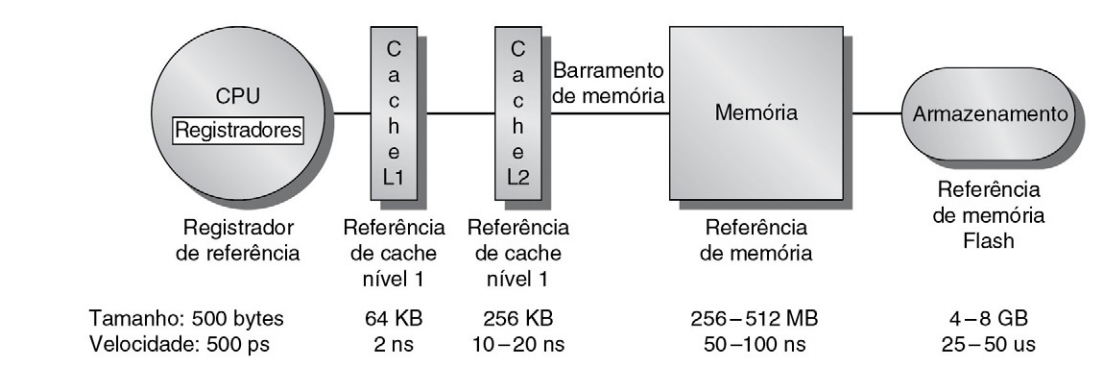
\includegraphics[width=\columnwidth]{images/mobile.png}}
  \footnotesize{Fonte: \citet{book-computer-architecutre}}
  \label{fig:hierarquia-de-memoria}
\end{figure}

Possuindo relação direta com a Teoria da Informação\footnote{Teoria matemática proposta inicialmente por Claude Shannon que busca quantificar a informação.}, uma estrutura de dados é dita sucinta se ela pode representar informações usando um espaço próximo à entropia\footnote{Número mínimo de bits necessários para diferenciar um objeto em um conjunto de dados.} determinada por essa teoria, que como mostra \citep{book-compact-data-structures}, 
em seu livro, no pior caso é de $\log_2 |U|$ bits para um objeto de cardinalidade $U$.
Além disso, essa estrutura deve fornecer suporte a uma série de operações primitivas sobre os seus objetos de modo eficiente. Por fim, uma estrutura de dados sucinta é considerada mais eficiente do que outros algoritmos de compactação clássicos, porque estes precisam descompactar os dados antes de operar sobre os mesmos, tornando inviável a manipulação de grandes conjuntos de dados em memórias como a cache e a RAM.


\section{Árvores Sucintas}
As árvores são uma das estruturas de maior sucesso na ciência da computação. Isso se deve ao fato de que essa estrutura é de simples compreensão e possibilita operações de busca, inserção e remoção de forma eficiente.
Uma árvore $T=(V,E)$ é uma estrutura de dados hierárquica, ou seja não linear, formada por vértices (V) e arestas (E). Assim, árvores são definidas também como grafos, sendo eles conexos, não dirigidos e acíclicos, 
ou seja para qualquer dois vértices em $T$ existe um único e simples caminho. \citep{book-algoritmos-teoria-pratica}.

Encontramos diversas aplicações construídas a partir destas estruturas, entre elas aplicações de banco de dados e tradutores de idiomas \citep{book-algoritmos-teoria-pratica}. Árvores também são amplamente usadas no campo de aprendizagem de máquina: são as chamadas árvores de decisão, que auxiliam desde a escolha do melhor movimento em um jogo de xadrez  à operações em sites de comércio eletrônico \citep{book-inteligencia-artificial}.
A \figref{fig:example-tree} exemplifica a forma gráfica de uma árvore que armazena a estrutura do domínio \textit{data.structure.trees.com} (DNS são organizados em árvores, tendo o seu sufixo armazenado na raíz) e parte da representação de  uma árvore de decisão de um jogo da velha.

\begin{figure}[!ht]
\centering
  \caption[Exemplos de representação gráficas de árvores]{Exemplos de representação gráficas de árvores}
  \subfigure[ref1][Árvore de DNS, a subárvore enraízada no nó \textbf{com} define o domínio \textit{data.structure.trees.com}]{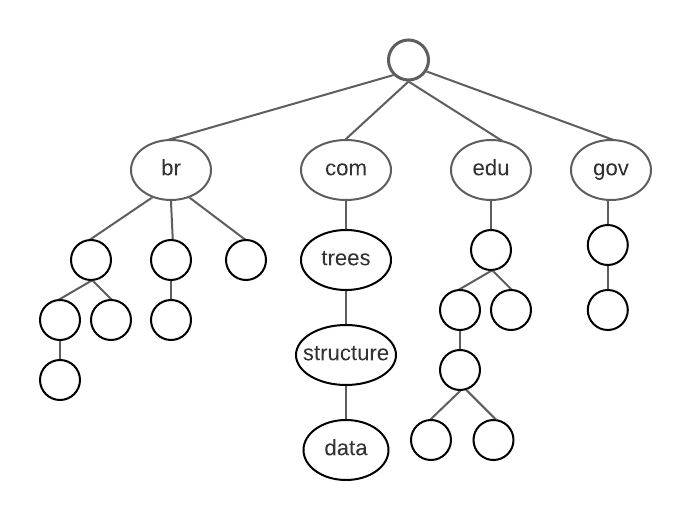
\includegraphics[scale=0.8]{images/tree-dns.png}}
  \qquad
  \subfigure[ref1][Segmento de uma árvore de decisão para um jogo da velha]{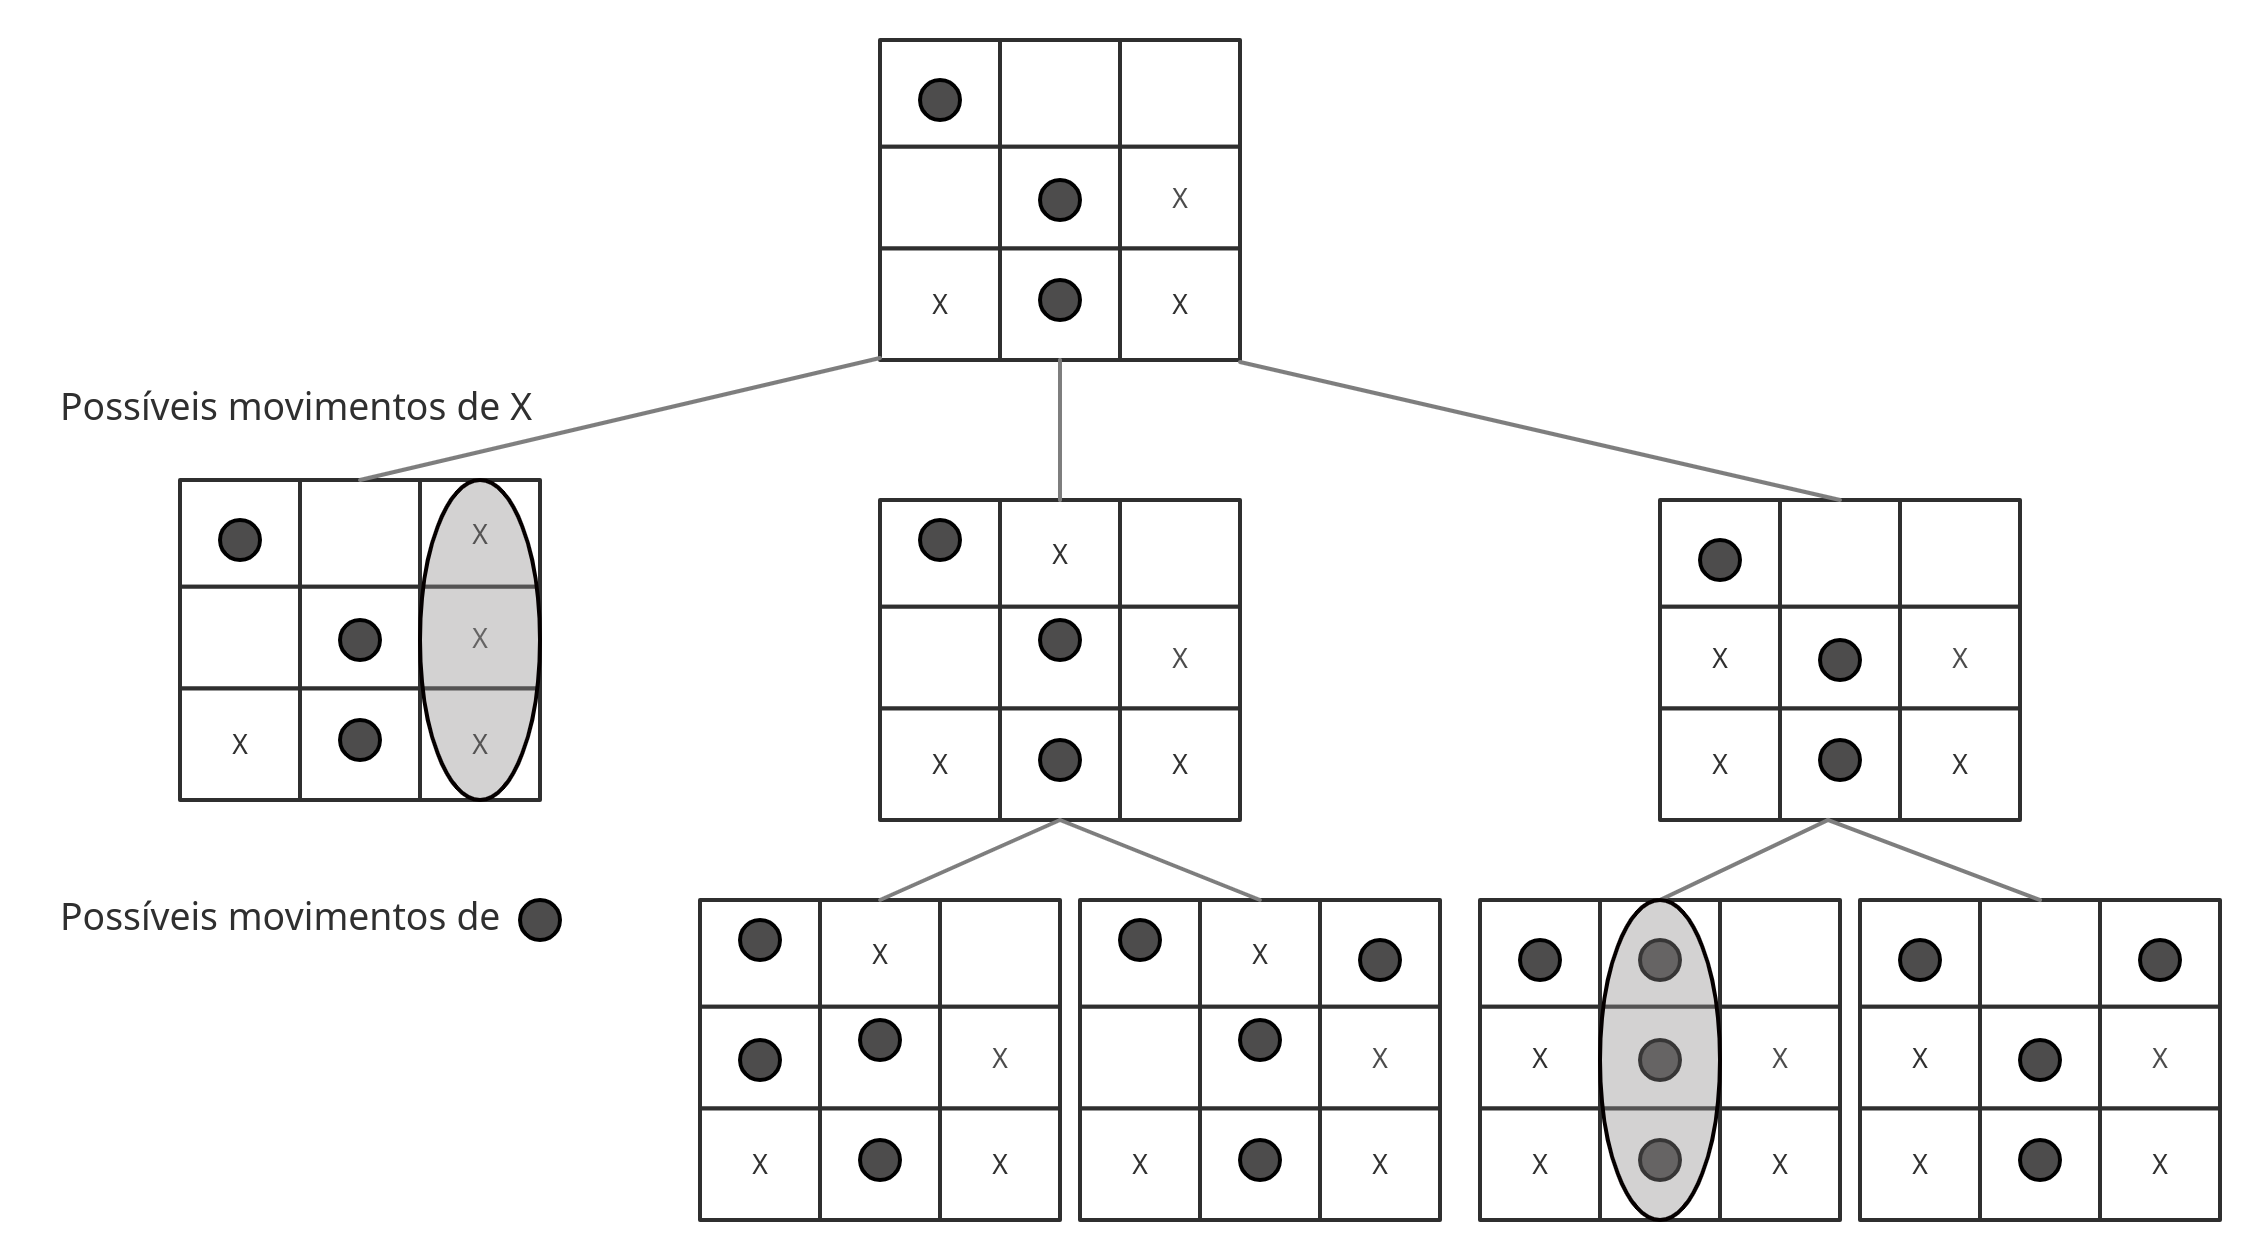
\includegraphics[width=\columnwidth]{images/decision-tree.png}}
  \label{fig:example-tree}
\end{figure}

Mas mesmo estruturas eficientes como as árvores podem se tornar inviáveis para determinadas aplicações. A forma como estas são construídas afim de operar sobre os objetos podem muitas vezes ocupar um espaço ainda maior do que os dados ocupariam originalmente. Para reconhecer este problema \citet{book-compact-data-structures} traz como exemplo uma comparação do espaço ocupado pelo genoma humano armazenado sem estruturas adicionais e o espaço ocupado pelo mesmo usando uma árvore de sufixos para
viabilizar operações de montagem de genomas. Com  3,3 bilhões de nucleotídeos, se usarmos 2 bits para armazenar cada base nitrogenada necessitaremos de aproximadamente 825 megabytes, assim podemos reter o DNA por completo em qualquer memória principal, no entanto, usando a árvore de sufixos, cada nucleotídeo precisará de 10 bytes para ser representado, o que nos leva a uma estrutura que ocupa um espaço igual à 33 gigabytes, o que torna inviável o processamento do genoma em memória principal na maioria dos computadores comuns. %Fazendo com que seja necessário armazenar parte do mesmo em memórias como o disco, o que como já vimos acarreta em um alto custo computacional.

É nesse ponto que entram as estruturas de dados sucintas. Como já vimos, estas são capazes de armazenar tanto as informações, como as estruturas de dados que atuam sobre elas usando um espaço reduzido. No caso das árvores que é o objeto do nosso estudo, a sua representação clássica com ponteiros  ocupa  $O(n \log n)$ bits\footnote{Neste
trabalho, quando não indicado, estaremos trabalhando com o logarítmo na base 2.}, enquanto existem representações sucintas, abordadas nas Seções \ref{sec:sec-bitvector} e \ref{sec:sec-parenthesis-balanceados}, que ocupam cerca de $2n+o(n)$ bits.

\section{Vetores de Bits}\label{sec:sec-bitvector}
Um vetor de bits $BP[0,n-1]$  é uma sequência sobre o alfabeto $\Sigma = \{0,1\}$. É interessante que as seguintes operações sejam executadas sobre os vetores de bits \citep{book-compact-data-structures}:

\begin{itemize}
    \item $access(BP,i)$: retorna o i-ésimo bit do vetor BP, com $0 \leq i < n$;
    \item $rank_v(BP,i)$: seja $v \in \{0,1\}$, e $0 \leq i < n$, esta operação retorna o número de ocorrências de $v$ no intervalo $BP[1,i]$.\\
    Sendo que a seguinte relação de equivalência é válida: $rank_0(BP,i)=i - rank_1(BP,i)$. Um caso particular dessa operação é $rank_v(BP,0)=0$;
    \item $select_v(BP,i)$: dado $v \in \{0,1\}$ e $0 \leq i < n$. $select$ retorna a posição do i-ésimo bit $v$ em $B$, sendo que assim como em $rank$ por definição $select_v(BP,0)=0$.
\end{itemize}

A \figref{fig:bitvector-operations} traz exemplos das operações listadas.
\begin{figure}[!ht]
\centering
  \caption[Operações sobre vetores de bits]{Operações de $rank, select$ e $access$ sobre $B=11010100$}
  \subfigure[Operação de $access$ sobre $B=11010100$][$access(BP,4)=1$]{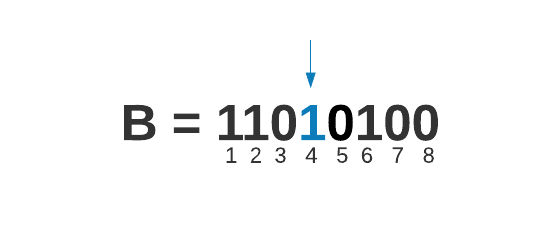
\includegraphics[scale=0.6]{images/access.png}}
  \subfigure[Operação de $rank$ sobre $B=11010100$][$rank_1(BP,6)=4$]{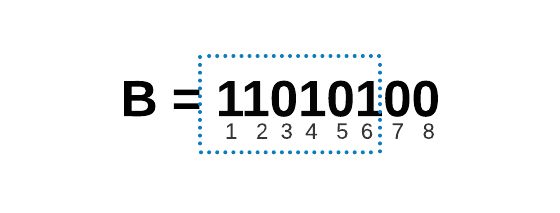
\includegraphics[scale=0.6]{images/rank.png}}
  \subfigure[Operação de $select$ sobre $B=11010100$][$select_0(BP,3)=7$]{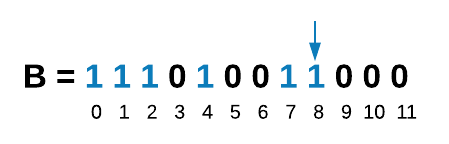
\includegraphics[scale=0.6]{images/select.png}}
  \label{fig:bitvector-operations}
\end{figure}

\section{Representação de árvores sucintas}
Existem diversas formas de representar  uma árvore de maneira sucinta, abaixo listamos algumas destas, sendo que o nosso foco neste trabalho será a primeira forma, representação sucinta via
parênteses balanceados.
\subsection{Parênteses Balanceado (BP)}\label{sec:sec-parenthesis-balanceados}
\begin{figure}[!ht]
\centering
  \caption[Representação de árvores com parênteses balanceados]{Representação de uma árvore geral $T$ usando parênteses balanceados: fazendo um percurso pré-ordem em $T$ escrevemos um parênteses de abertura quando um nó é visitado pela primeira vez, e um de fechamento no percurso de volta após atravessar sua subárvore \citep{paper-succint-representation-of-balanced-parentheses}}
  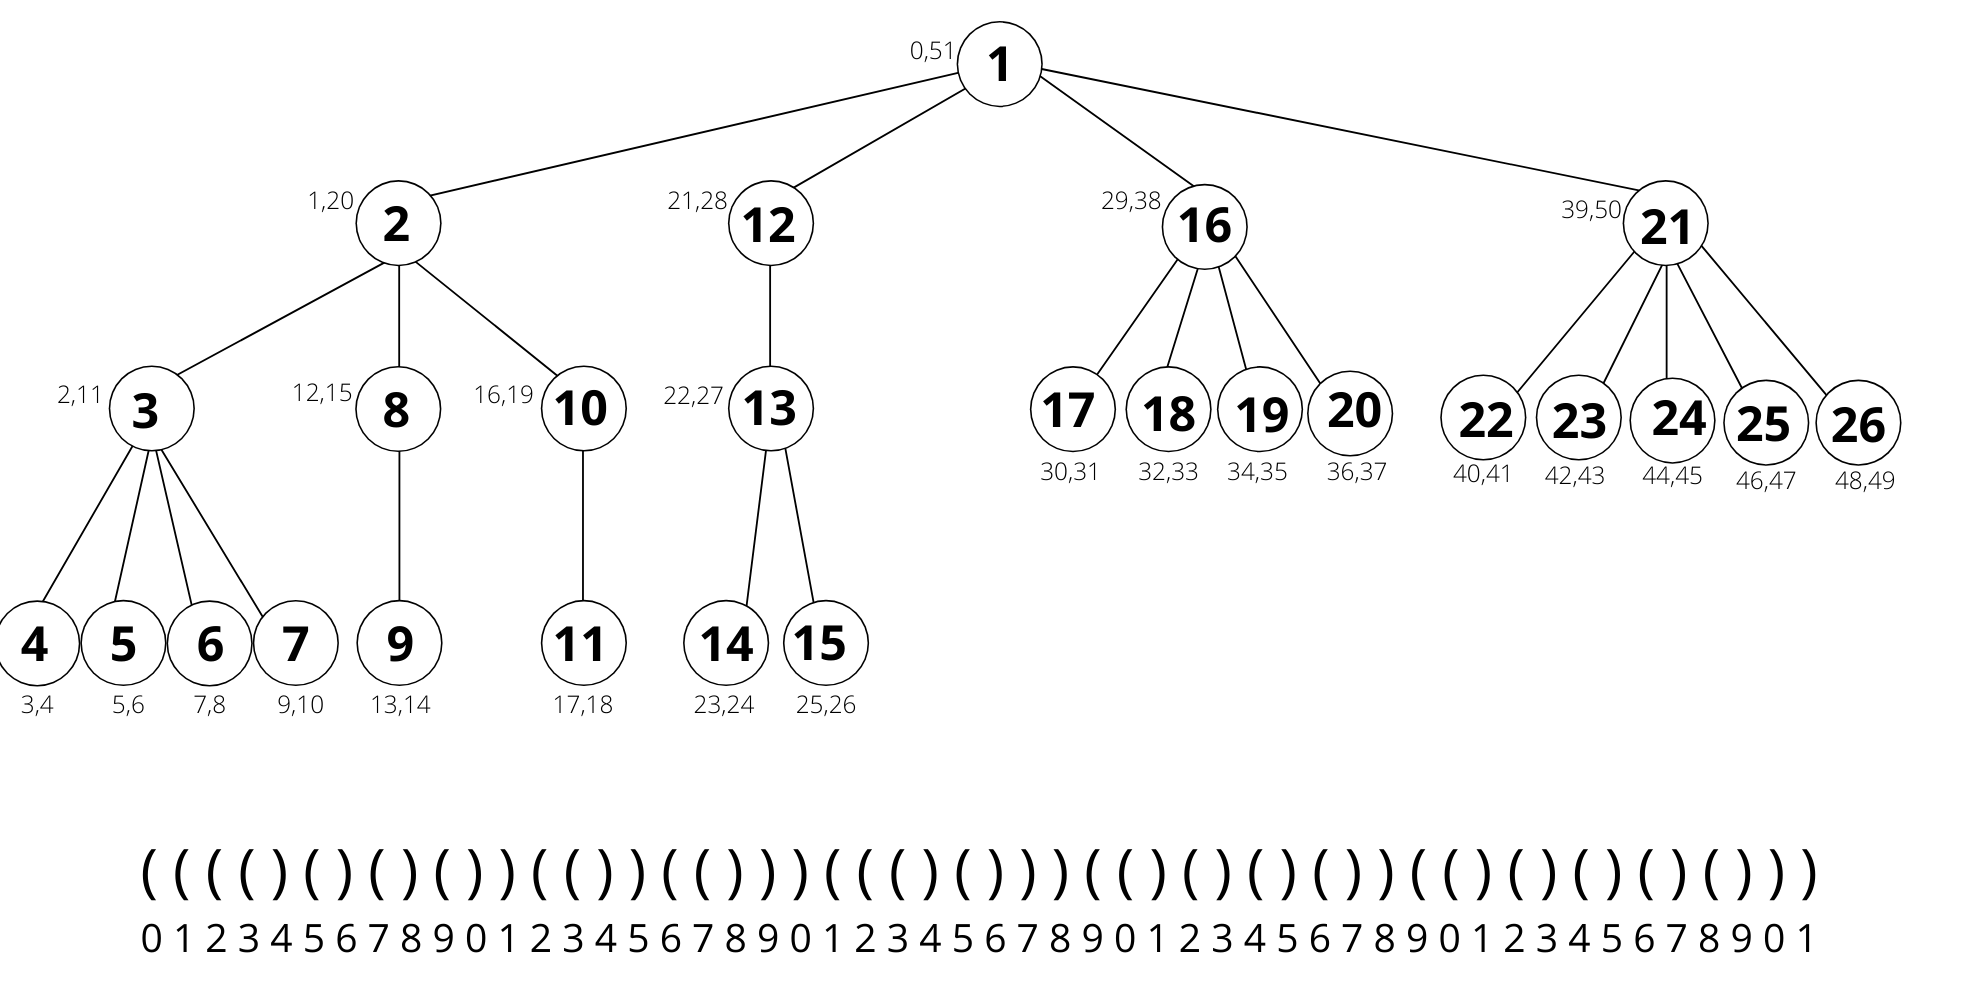
\includegraphics[width=\columnwidth]{images/arvore_geral.png}
  \label{fig:parenthesis-representation}
\end{figure}
Uma sequência de parênteses balanceados (BP) consiste em uma string de tamanho igual à $2n$, sendo $n$ parênteses de abertura '(', e $n$ parênteses de fechamento ')'. Essa estrutura descreve uma relação de hierarquia/contenção, e portanto é amplamente utilizada para a representação de árvores.

Para representar um árvore ordinal $T$ usando essa estrutura, tomamos um vetor de bits de tamanho igual à $2n$ ($BP[0,2n-1])$, onde $n$ é o número de nós da árvore. Realizamos então um percurso sobre $T$ em pré-ordem, e sempre que um nó for alcançado pela primeira vez, um parênteses de abertura (representado pelo bit $1$) é inserido em $BP$, ao término da exploração das subárvores deste nó, um parênteses de fechamento (bit $0$) é inserido em $BP$ \citep{paper-succint-trees-in-practice}.  Na figura \figref{fig:parenthesis-representation} vemos uma árvore com 26 nós e sua representação equivalente em parênteses balanceados.
%Para representar uma árvore ordinal $T$ usando essa estrutura tomamos um vetor de tamanho igual à $2n$ ($BP[0,2n-1])$ onde $n$ é o número de nós da árvore. O nó $v$ (codificado em $BP[i]$) da árvore $T$ é representado por um parênteses de abertura e um de fechamento em $BP$, os elementos contidos no intervalo aberto desses parênteses codificam as subárvores de $v$ em ordem de igual maneira. Na figura \figref{fig:parenthesis-representation} vemos um árvore com 14 nós e sua representação equivalente em parênteses balanceados.

Usando a representação de parênteses balanceados, podemos fornecer suporte às operações a seguir para diversas estruturas de dados sucintas:
\begin{itemize}
    \item $findclose(BP,i)$: retorna a posição $j$ do parênteses de fechamento correspondente ao i-ésimo parênteses de abertura;
    \item $findopen(BP, i)$: retorna a posição $j$ do parênteses de abertura correspondente ao i-ésimo parênteses de fechamento;
    \item $excess(BP, i)$: retorna a "diferença entre o número de parênteses abertos e fechados até a posição $i$".  \cite[tradução nossa]{paper-succint-representation-of-balanced-parentheses}
\end{itemize}

\citet{paper-succint-representation-of-balanced-parentheses} proporam uma solução em árvores binárias usando a representação de parênteses balanceados, onde  além das operações já citadas, oferece também suporte a operação de $enclose(i)$, que retorna o pai do nó $i$, 
e a operação $double\_enclose(i,j)$ (que equivlae à operação $lca$ em árvores) que por sua vez retorna o pai dos nós $i$ e $j$. 

Através da operação  $rank$ podemos viabilizar a operação de $excess$ facilmente, como mostrado abaixo.

\begin{eqnarray*}
    \begin{split}
        excess(BP,i) &= rank_1(BP,i) - rank_0(BP,i) \\
        &  = rank_1(BP,i) - (i - rank_1(BP,i)) \\
        &  = 2 \cdot rank_1(BP,i) - i 
    \end{split}
\end{eqnarray*}

Por fim, através das operações definidas em vetores de bits e parênteses balanceados podemos fornecer suporte às diversas operações sobre árvores, como a obtenção do tamanho da subárvore de um
nó $i$, que pode ser feita através de: $(findclose(BP,i)+i-1)/2$. Esta expressão retornará a quantidade de nós codificados dentro do intervalo de contenção de $i$. Podemos ainda averiguar se um
nó $j$ da árvore é ou não um nó folha, bastando verificar se o elemento que segue imediatamente à $j$ é um parênteses de fechamento, isso pode ser feito através da operação de $access(BP,j+1)$,
que irá retorna o $k$-ésimo bit de $BP$, com $k=j+1$.

\subsection{Unary Degree Sequence (DFDUS)}
Outra forma de representar árvores é atráves da \textit{Sequência de grau unário}, que também faz o uso de uma travessia pré-ordem (como BP) para construir a árvore.
A diferença é que a para codificar um nó, inserimos $i$ parênteses de abertura (onde $i$ é o número de filhos deste nó) e $1$ parênteses de fehcamento. 
Desse modo, conforme afirma \citeauthor{paper-succint-trees-in-practice}, "o nó passa a ser representado pela posição de seus $i$ parênteses". 
O autor mostra que a sequência resultante ainda é balanceada, se adicionarmos um parênteses de abertura ao ínicio da mesma. A \figref{fig:dfdus-representation}, mostra a representação equivalente
à de parênteses balanceadas, com \textit{DFDUS} para  a árvore geral mostrada acima.
\begin{figure}[!ht]
    \centering
      \caption[Representação de árvores com Sequência de Grau Unário]{Representação de uma árvore geral $T$ usando DFDUS}
      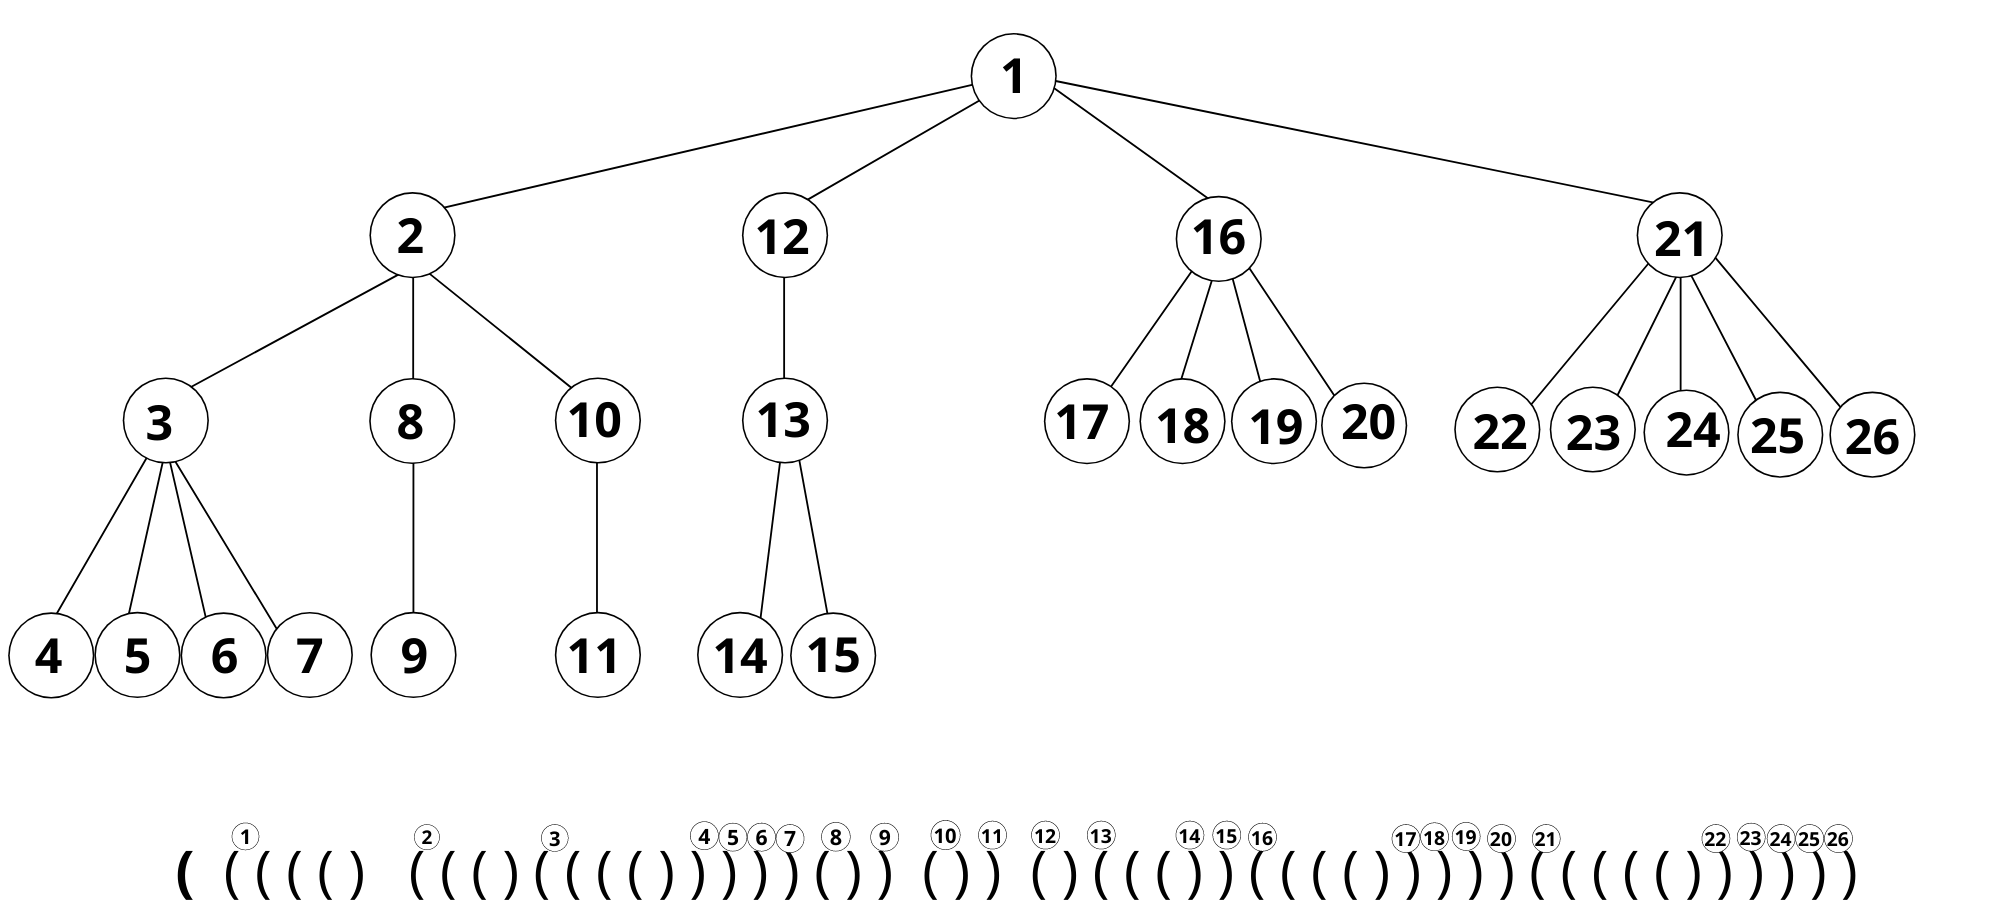
\includegraphics[width=\columnwidth]{images/dfdus.png}
      \label{fig:dfdus-representation}
\end{figure}

\subsection{Level-ordered Unary Degree Sequence (LOUDS)}
Nesta representação, pecorremos os nós em largura, adicionando assim como em \textit{DFDUS} $i$ parênteses de abertura ao visitarmos um nó pela primeira vez, e $1$ parênteses de fechamento.
Novamente com $i$ represetando o número de filhos daquele nó.

\section{Range min-Max Tree}\label{sec:sec-classic-rmm-tree}
A Range min-Max-tree (rmM-tree) é construída na forma de uma árvore binária completa (o que nos permite usar uma heap\footnote{"Objeto arranjo que pode ser visto como uma árvore binária quase,
onde cada nó da árvore corresponde a um elemento do arranjo." \citet{book-algoritmos-teoria-pratica}} sem ponteiros), onde cada um de seus nós armazenam valores de excesso calculados dentro de um intervalo de um vetor da representação de parênteses balanceados. Esse vetor deve representar a relação de contenção dos nós da árovre ordinal sobre a qual devemos operar, para tanto podemos usar a estrutura de vetores de bits ou a de parênteses balanceados  que expomos anteriormente na \figref{fig:parenthesis-representation}. 

A construção da rmM-tree segue uma abordagem \textit{bottom-up}, onde a cada nó, calcula-se primeiro o intervalo a ser coberto, para então definir os  valores de excesso. Após construir os nós folhas dessas estrutura, repetimos o processo descrito para os nós internos (e raíz), sendo que o intervalo coberto por cada nó é a união de área de seus nós filhos.


%A quantidade de intervalos armazenados por essa estrutura influência diretamente na complexidade de espaço ocupado pela mesma. 
Como cada nó folha está associado a um único intervalo, o tamanho dessa estrutura está também relacionada a quantidade e ao tamanho dos intervalos cobertos pela mesma. 
Esses intervalos são obtidos da seguinte maneira, dado um vetor de entrada $BP$, de  tamanho igual à $n$, sendo $BP$ usado para a codificação de uma árvore ordinal $T$, é definido um tamanho de intervalo $b$ (chamado também de tamanho de bloco), e então divide-se $n$ por $b$, obtendo assim a a quantidade de folhas da rmM-tree.
Considerando que a altura de uma árvore binária é dada por $\lceil \log n \rceil$ e que o vetor de entrada $B$ ocupa $n$ bits, temos assim que a rmM-tree tem uma ocupa um espaço próximo à $n + O(\frac{n}{b} \log n)$ bits, fazendo $b = \log^2 n$, temos uma complexidade de espaço igual à $n + O(n/\log n)$. Por fim,  como mostra \citet{book-compact-data-structures} 
em seu livro, na prática todas as operações sobre a rmM-tree podem ser realizadas em tempo $O(\log n)$ - ou ainda em tempo $O(\log \log n)$ em uma versão mais refinida da estrutura - a lista completa dessas operações é apresentada na \tabref{tbl:classicOperations-rmm-tree} deste capítulo.
%TODO: b é fixado em log^2n, o que nos dá $n + O(\frac{n}{\log n}$ bits$

\subsection{Registros}
Os valores de excesso definido em cada nó da rmM-tree são essenciais para a realização de operações de consulta de maneira eficiente, são neles em que essa estrutura se baseia.  Em seu livro, \citeauthor{book-compact-data-structures} ,
define 4 valores de excesso que viabilizam essas operações. Mostraremos as definições de cada um destes a seguir. Suponha que um nó $v$ cubra um intervalo $[s,e]$ do vetor de entrada $BP$ de parênteses balanceados, define-se então:
\begin{itemize}
    \item \textit{R[v].e}: excesso total no intervalo $[s,e]$
    
    $R[v].e = excess(e) - excess(s-1)$.
    \item \textit{R[v].m}: excesso mínimo local
    
    $R[v].m = \min\{excess(i) - excess(s - 1) | s \leq i \leq e\}$.
    \item \textit{R[v].M}: excesso máximo local
    
    $R[v].M = \max\{excess(i) - excess(s - 1) | s \leq i \leq e\}$.
    
    \item \textit{R[v].n}: é definido pelo número de vezes que o excesso mínimo ocorre dentro do intervalo coberto. Assim, suponha $m$ o vetor de excessos sobre o intervalo $[s,e]$, então:
    $R[v].n = |\{BP[i]=R[v].m | s \leq i \leq e\}|$
    %$R[v].n= |{p \in BP[s,e], excess(p) - excess(s - 1) = R[v].m}|$
\end{itemize}

    Agora que temos a definição de cada campo da Range min-Max tree (estas definem os valores dos nós folhas), podemos analisar a construção de seus nós internos. Como já dito, estes nós são construídos  a partir da união das áreas cobertas por seus nós filhos, e como nossa estrutura é construída através de um vetor, sabemos que os filhos de um nó $v$ é dado pelos nós $2v+1$ e $2v + 2$, isso nos leva as seguintes recorrências:
    \begin{itemize}
        \item $R[v].e = R[2v +1 ].e + R[2v + 2].e$
        \item $R[v].m = min(R[2v+1].m, R[2v+1].e + R[2v + 2].m)$
        \item $R[v].M = max(R[2v+1].M, R[2v+1].e + R[2v + 2].M)$
        \item $ R[v].n =
           \begin{cases}
                 R[2v+1].n, & \mbox{se } R[2v+1].m < R[2v+1].e + R[2v + 2].m; \\
                 R[2v + 2].n, & \mbox{se } R[2v+1].m > R[2v+1].e + R[2v + 2].m; \\
                 R[2v+1].n + R[2v + 2].n, & \mbox{se }  R[2v+1].m = R[2v+1].e + R[2v + 2].m .
           \end{cases}
        $
    \end{itemize}
\begin{example}\label{ex-build-tree}
    Para melhor elucidar a construção dessa estrutura usaremos o exemplo da Seção~\ref{sec:sec-parenthesis-balanceados} e demonstraremos o cálculo dos campos e dos intervalo de um nó folha, 
    mostraremos também como é construído os campos de  um dos nós internos da rmM-tree. No exemplo em questão, temos um vetor de entrada com 52 parênteses balanceados, 
    definiremos um tamanho de bloco $b=4$, o que implica que a árvore terá:

    \begin{itemize}
        \item $r = n/b \to r = 52/4 = 13 $ folhas;
        \item 12 nós internos, pois $r-1 = 12$;
        \item Altura $h= \ceil{\log r} \to h = \ceil{\log 13}= 4$;
        \item Como o número de folhas não é uma potência de 2, temos que as folhas $0$ até $2*r - 2^h  -1 = 9$ estão agrupadas no último nível da árvore,  e as outras $2^h - r = $ folgas estão agrupadas à
        direita no nível anterior.
    \end{itemize}

    Assim temos os seguintes valores para a folha $0$ (nó $15$) da árvore:
        \begin{itemize}
            \item  Área de cobertura:
            $ [(i-1)\cdot b +1, i\cdot b] = [1,4]$
            \item Excesso global:
            $R[15].e = excess(4) = 2 \cdot rank_1(BP,4) - 4 = 4 
            $
            \item Excesso mínimo:
            $R[15].m = min(1,2,3,4) = 1$
            \item Excesso máximo:
            $R[7].M = max(1,2,3,4) = 4$
            \item Número de vezes que o excesso mínimo ocorre no intervalo:\\
            $R[7].n = count((1,2,3,4),1) = 1$
        \end{itemize}
        
    Mostraremos agora o cálculo do 7º nó interno do nosso exemplo, este cobre as folhas 0 e 1 da árvore (nós 15 e 16, respectivamente), com base nas definições anteriores temos então:
    \begin{itemize}
        \item Área de cobertura: $BP[1,4] \cup BP[5,8]$
        \item Excesso global: \\
        $R[7] = R[15].e + R[16].e = 4 + 0 = 4$
        \item Excesso mínimo:\\
        $R[7].m = min(R[15].m, R[15].e+R[16].m) = (1,4-1)=1$
        \item Excesso máximo:\\
        $R[7].M = max(R[15].M, R[15].e+R[16].M) = (4,4+0)=4$
        \item Número de vezes que o excesso mínimo ocorre no intervalo:\\
        $R[7].n = R[15].n = 1$ pois $R[15].m < R[15].e+R[16].m$
    \end{itemize}

    O processo mostrado acima deve ser repetido para os demais nós da árvore até que cheguemos a raíz, dando origem a árvore mostrada na \figref{fig:rmm-tree-binaria}. 
    \begin{figure}[!ht]
     \centering
      \caption[rmM-tree clássica.]{rmM-tree clássica,com tamanho de bloco igual à 4. A estrutura foi construída a partir dos 52 parênteses balanceados mostrados na parte inferior}
      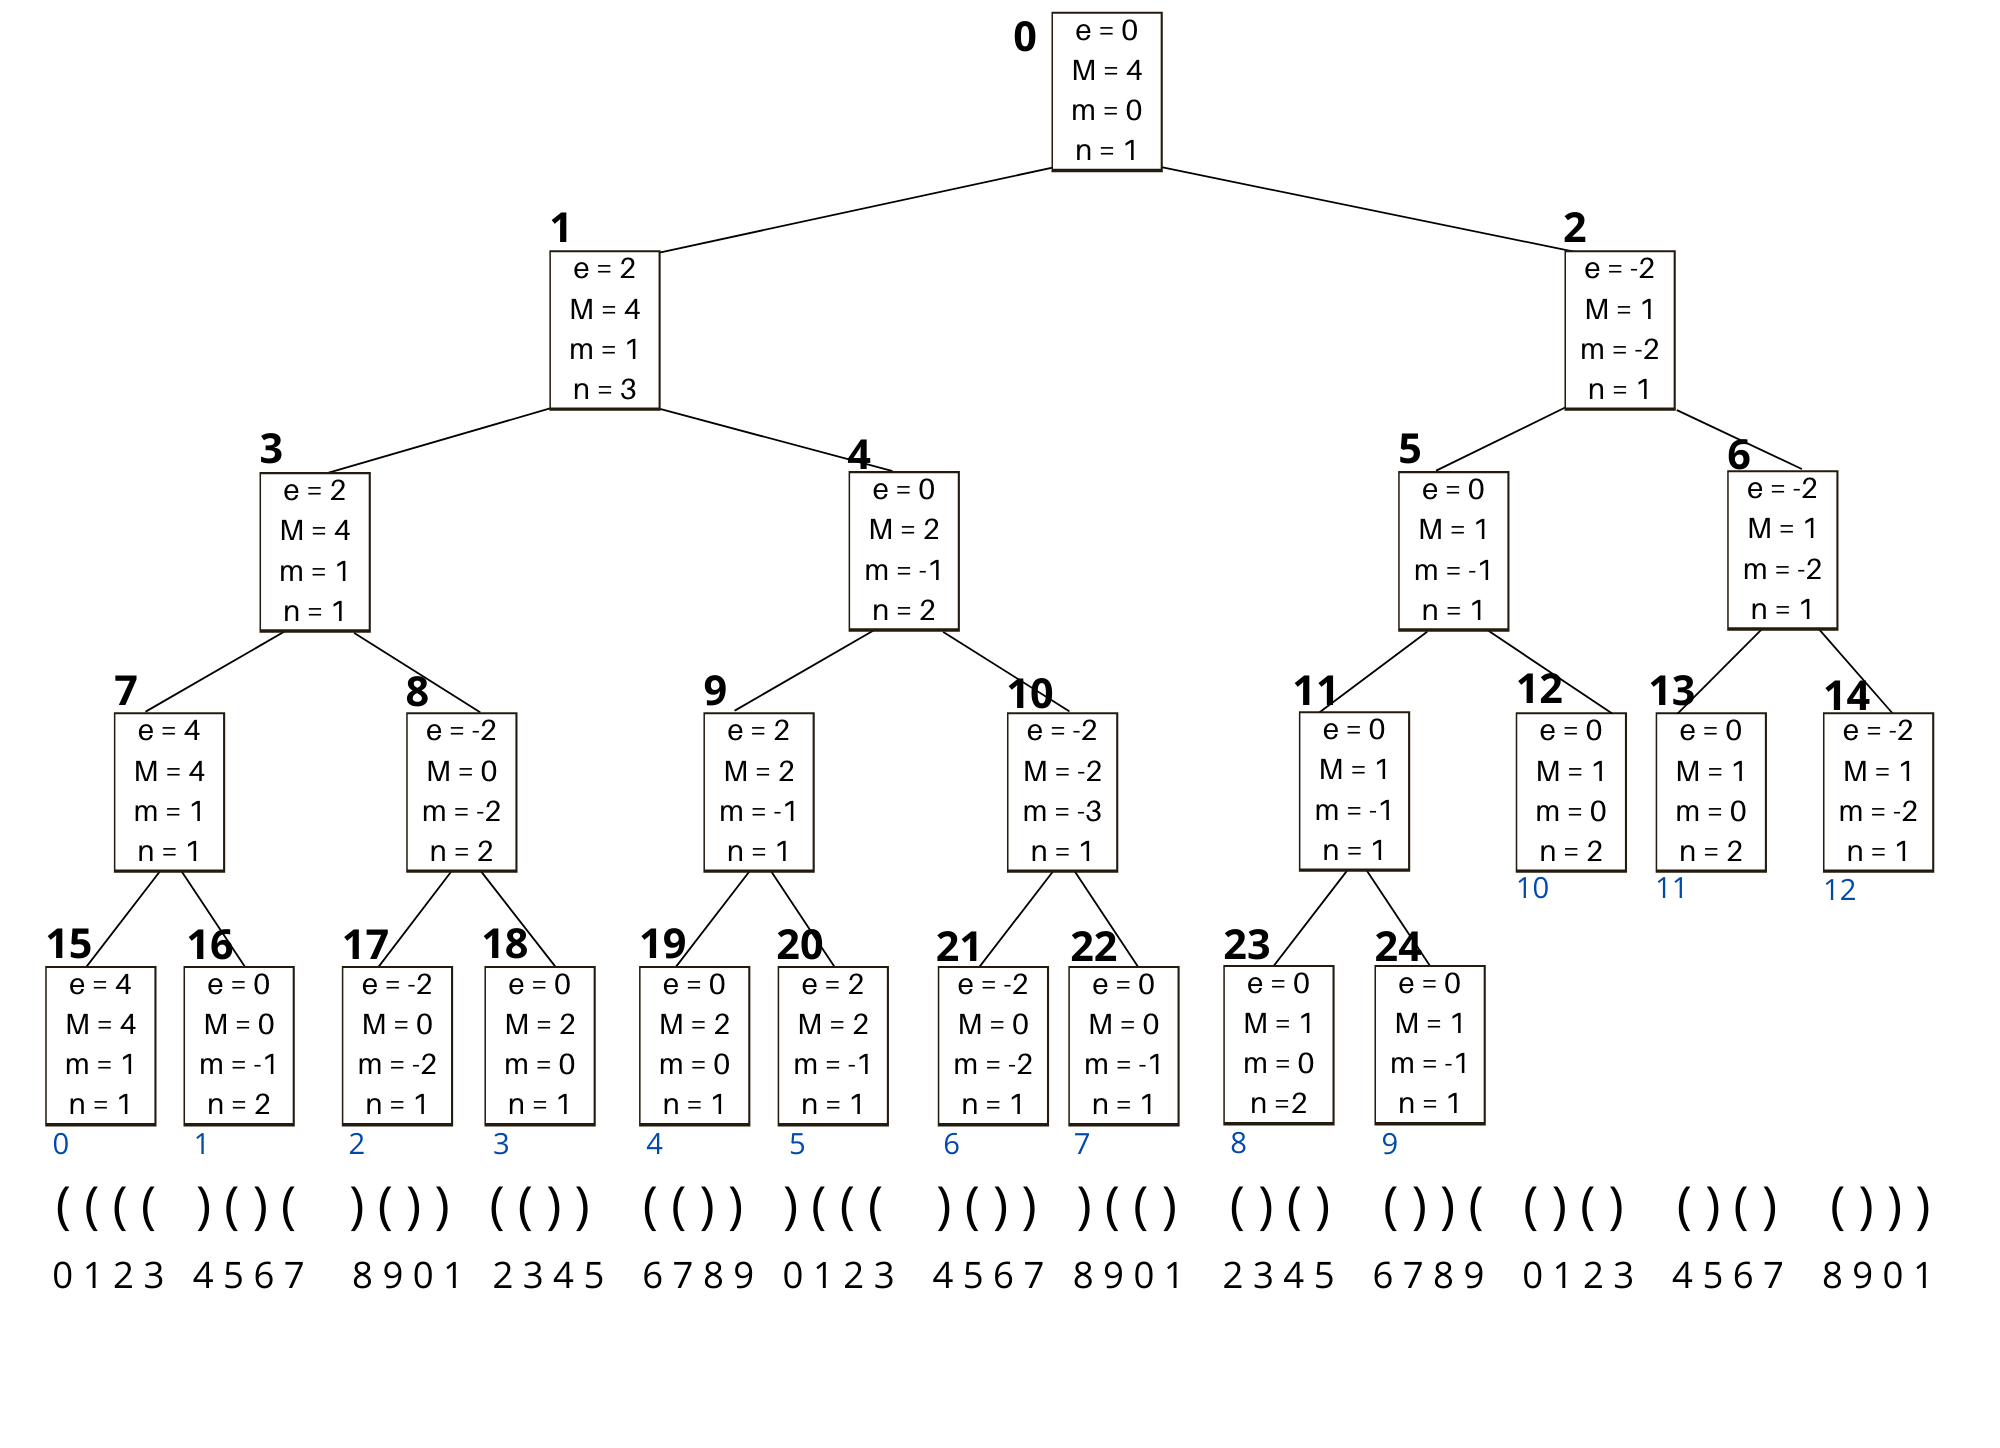
\includegraphics[width=\columnwidth]{images/rmm-tree-bin.png}
      \label{fig:rmm-tree-binaria}
    \end{figure}
\end{example}

O processo de construção da rmM-tree é mostrado com mais detalhes no algoritmo~\ref*{alg:build-bin-tree}.
No algoritmo apresentado, usamos uma tabela $C$, o uso dessa tabela não é obrigatório, mas ela otimiza o tempo gasto para construir e operar sobre
a rmM-tree, como mostra \citeauthor{book-compact-data-structures}. A construção desta, se dá do seguinte modo, define-se primeiro uma constante 
$w$, tal que $b \mbox{ mod } w = 0$, e cria-se então uma tabela $C[0, 2*w]$, 
onde cada entrada da tabela armazena valores excesso definidos pela estrutura da rmM-tree, cada elemento $C[x]$ é calculado com base nos $w$ bits 
que formam $x$. 
\begin{example}
    Suponha $w=4$ e $x=3$, temos assim que:

    $$3_2 = 0011,$$  logo:
    \begin{itemize}
        \item $C[x].e = 0; C[x].M = 0; C[x].m = -2; C[x].n = 1$
    \end{itemize}
\end{example}

Fazer a pré-computação dessa tabela elimina a necessidade computar iterativamente os valores de excesso mínimo e máximo, a cada inspeção de bits.
Assim, no momento da construção dos nós folhas, ou durante a inspeção dos bits que a compõe, basta ler os $w$ bits que queremos inspecionar, convertêr-los 
para a base $2$, e então realizar uma consulta na tabela $C$, que conforme mostra \citet{book-compact-data-structures} leva tempo $O(\frac{n}{\log n})$.   
A função \textit{bitsread}, atua junto à tabela $C$ otimizando o tempo de resposta das nossas operações, e por esse motivo é usada durante todo o nosso 
projeto, ela recebe como parâmetro um índice $i$, e lê $i$ e os $w-1$ bits seguintes no vetor de bits de entrada, 
após a leitura desses $w$ bits está função os converte da forma binária para decimal, e usa o valor obtido para consultar na tabela $C$ os valores de excesso 
correspondentes aos bits analisados. Além da tabela $C$ e da função \textit{bitsRead}, em nossa implementação usamos outras duas funções que nos auxiliam no 
percurso em árvore, denominadas \textit{leafInTree}
e \textit{numLeaf}, a primeira retorna o índice de um nó na rmM-tree correspondente ao número de uma folha, a segunda por sua vez retorna o número de uma folha 
correspondente à um nó da rmM-tree.

\begin{example}
    Tome com base agora, a nossa rmM-tree de exemplo, assuma $w=2$, e suponha que queremos construir a folha de número $0$ (nó $15$), 
    o intervalo que a folha $0$ cobre vai de $0$ à $4$, assim precisaríamos ler os $4$ bits que compõe esse intervalo, para um exemplo pequeno como 
    este não há problemas em calcular esses valores iterativamente, mas imagine o que acontece com casos em que temos uma árvore de entrada maior, 
    e um tamanho de  blocos também maior, o processo se tornaria mais oneroso. Observe então como este processo é feito usando a tabela de excessos $C$.


    \begin{itemize}
        \item Como $w=2$, convertemos primeiro os bits codificados em $BP[0,1]$\\
        $BP[0,1] = 11$ que em decimal corresponde à $3$\\
        Fazemos então uma consulta na tabela $C$, na posição $3$, que conforme explicamos anteriormente, traz os seguintes valores:
        $$C[3].e = 2; C[3].M = 2; C[3].m = 1; C[3].n=1.$$
        Nesse momento, os valores de registro para nossa folha são:\\
        $$R[15].e = 2; R[15].M = 2; R[15].m = 1; R[15].n=1.$$
        \item  Agora precisamos computar os valroes correspondentes aos $w$ bits restantes que compõe a nossa folha, temos que:
        $BP[3,4] = 11$ que em decimal corresponde à $3$\\

        Agora que sabemos a que elemento em $C$ essa parcela da nossa folha corresponde, podemos obter os valores de excesso para o intervalo completo da folha,
        imagine que estamos unindo dois intervalos coberto por um nó pai. Temos assim que:
        \begin{itemize}
            \item $R[15].e = R[15].e + C[3].e = 2 + 2 = 4$
            \item $R[15].M = max(R[15].M, R[15].e + C[3].M) =  max(2,2+2) =4$
            \item $R[15].m = min(R[15].m, R[15].e + C[3].m) = min(1,2+1) = 1$
            \item $R[15].n=1.$
        \end{itemize}
    \end{itemize}
\end{example}


\begin{algorithm}[h!]
    \Input{Vetor de bits $BP[0,n-1]$, tabela de excessos C, tamanho de bloco $b$ e de sub-bloco $w$, número de folhas $r$, quantidade de nós $nNodes$ }

    \tcp{Construção dos nós folhas}
    \For{$k \leftarrow 0$ \textbf{to} $r-1$}{
        $v \leftarrow leafInTree(k)$\\
        $R[v].e \leftarrow 0; R[v].m \leftarrow -w; R[v].M \leftarrow w; R[v].n \leftarrow 0 $\\
        \For{$p \leftarrow (k*(b/w))+1$ \textbf{to} $((k+1)*b)/w$}{
            $x \leftarrow bistread((p-1)*w)$;
            \lIf{$R[v].e + C[x].M > R[v].M$}{$R[v].M \leftarrow R[v].e + C[x].M$}
            \lIf{$R[v].e + C[x].m < R[v].m$}{$R[v].m \leftarrow R[v].e + C[x].m$}
            \ElseIf{$R[v].e + C[x].m = R[v].m$}{$R[v].n \leftarrow R[v].n + C[x].n$}
            $R[v].e \leftarrow R[v].e + C[x].e$
        }
    }

    \tcp{Construção dos nós internos e raíz}
    \For{$v \leftarrow nNodes - r -1 $ \textbf{to} $0$}{
        $vL \leftarrow (2*v)+1; vR \leftarrow vL + 1$\\
        $R[v].e \leftarrow R[vL].e + R[vR].e$\\
        \SetAlgoLined
        $R[v].M \leftarrow max(R[vL].M, R[vL].e + R[vR].M)$\\
        \SetAlgoLined
        $R[v].m \leftarrow min(R[vL].m, R[vL].e + R[vR].m)$\\
        \lIf{$R[vL].m > R[vL].e + R[vR].m$}{$R[v].n \leftarrow R[vR].n$}
        \lElse{$R[v].n \leftarrow R[vL].n + R[vR].n$}
    }
    \caption{Construção da range min-Max tree binária}
    \label{alg:build-bin-tree}
\end{algorithm}

\subsection{Operações}
As operações sobre a range min-Max tree são realizadas através de cálculos usando os valores de excessos definidos acima. 
Parte dessas já foram descritas nas Seções \ref{sec:sec-bitvector} e \ref{sec:sec-parenthesis-balanceados}, como as operações  $enclose, findclose, findopen, rank \mbox{ e } select$.
As mesmas possibilitam a derivação de diversas outras operações, e portnato reduzem de modo eficiente a quantidade de estruturas
necessárias para realziar diversas opeações de percurso em árvores.
Mas além das operações mostradas, existem outras importantes operações suportadas pela rmM-tree, detalhamos algumas logo abaixo, e
a tabela~\ref{tbl:classicOperations-rmm-tree} mostra a lista completa das operações suportadas pela nossa implementação da range min-Max tree binária.

\subsection{FwdSearch}
    O objetivo da operação \textit{forward search} (busca à frente), é encontrar um excesso relativo $d$, em relação à um nó codificado por um índice $i$ no vetor que 
    representa uma árvor geral. Desse modo, \textit{ fwdSearch} retorna um índice $j>i$, mais à esquerda possível de $i$, tal que, o nó definido por $j$ está à uma profundidade $d$ em relação ao nó codificado por $i$, o resultado 
    dessa operação é dado pela expressão abaixo:
    $$fwdsearch(i,d) = min\{j > i | excess(j) = excess(i) + d\}$$
    
    Como veremos a seguir, dessa operação deriva-se diversas outras, tais como \textit{findclose, lca (menor ancestral comum)} e outras operaçõess de percurso em árvore.

%alterar estilo do modo matemático: colocar mathrm, textsc
    \citet{paper-simple-and-efficient-fully-functional-succinct-trees} descrevem o funcionamento dessa operação da seguinte maneira: 
    dado um excesso desejado $d$, e um índice $i$, a partir do qual a busca dever ser feita, examinamos a folha $k$ (com $k= \ceil{i/b}$) 
    cujo o intervalo de cobertura engloba o índice $i$, a partir de $i+1$.
    Caso não encontremos $d$ dentro desse intervalo, usamos os nós da rmM-tree para encontrar o bloco do vetor de entrada a qual $d$ pertence.
    O processo para encontrar $d$ neste caso deve ser feito do seguinte modo:
    \begin{enumerate}
        \item Defina uma variável $dr$, iniciada em zero, está variável será responsável por armazenar o excesso local de cada bloco lido.
        Quando a busca por $d$ em um intervalo não obtiver sucesso, atualize o excesso computado até o momento, que é guardado em $dr$ 
        (basta adicionar à $dr$ o campo de excesso referente ao nó inspecionado, seguindo as regras do ponto $2$);
        \item Verifique se o nó analisado é um filho à esquerda ou um filho à direita.
        \begin{enumerate}
            \item Caso o nó seja um filho à esquerda, verifique se $d$ está contido no intervalo de excesso máximo e mínimo do seu irmão à 
            direita ($dr + v.direita.m \leq d \leq dr + v.direita.M$); se essa condição não for satisfeita atualize o valor de $dr$ (pelo ponto $1$) 
            e avance no percurso da rmM-tree através do pai do nó verificado;
            \item Se o nó analisado for um filho à direita, simplesmente atualize o índice do nó corrente para pai de $v$, sem atualizar $dr$.
        \end{enumerate}
        \item Prossiga recursivamente até que a condição $dr + v.direita.m \leq d \leq dr + v.direita.M$ seja cumprida, quando isso acontecer significa que encontramos o intervalo em que $d$ está contido;
        \item Afim de reduzir o intervalo de busca e encontrar o índice $j$ de modo mais eficiente, iniciamos o percurso de descida em árvore através de $v.direita$ (esse processo reduzirá o tamanho de intervalo, sem excluir a resposta), 
        seguindo pelo seu filho :
        \begin{enumerate}
            \item esquerdo, sempre que o excesso relativo $d$ estiver no intervalo de contenção dos seus campos de excessos máximos e mínimo;
            \item direito, sempre que a condição anterior não for satisfeita, nesse caso precisamos atualizar o valor de $dr$ pelo ponto $a$.
        \end{enumerate}
         \item O processo descrito é repetido até que cheguemos a um nó folha, então procuramos pelo excesso relativo $dr$ (atualizado ao longo do percurso) no bloco da folha em que nos encontramos. A primeira posição em que ocorrer este ecesso é a resposta para $fwdsearch$.
    \end{enumerate}
    
    O exemplo~\ref*{ex:bin-fwdSearch} demonstra o processo acima, e o algoritmo~\ref*{alg:fwdSearch-bin} fornece mais detalhes de como todo esse processo é feito:
    \begin{example}\label{ex:bin-fwdSearch}

        Dado um nó em $BP$, codificado em $i=21$, encontrar o primeiro índice $j>i$,tal que $excess(j) - excess(i) = -1$.


        A \figref{fig:bin-fwdSearch}, destaca os bits, registros e índices dos nós inspecionados.
        \begin{figure}[h!]
           \centering
             \caption[fwdSearch(21,-1).]{Simulação da operação \textit{fwdSearch(21,-1)} em uma rmM-tree binária.}
             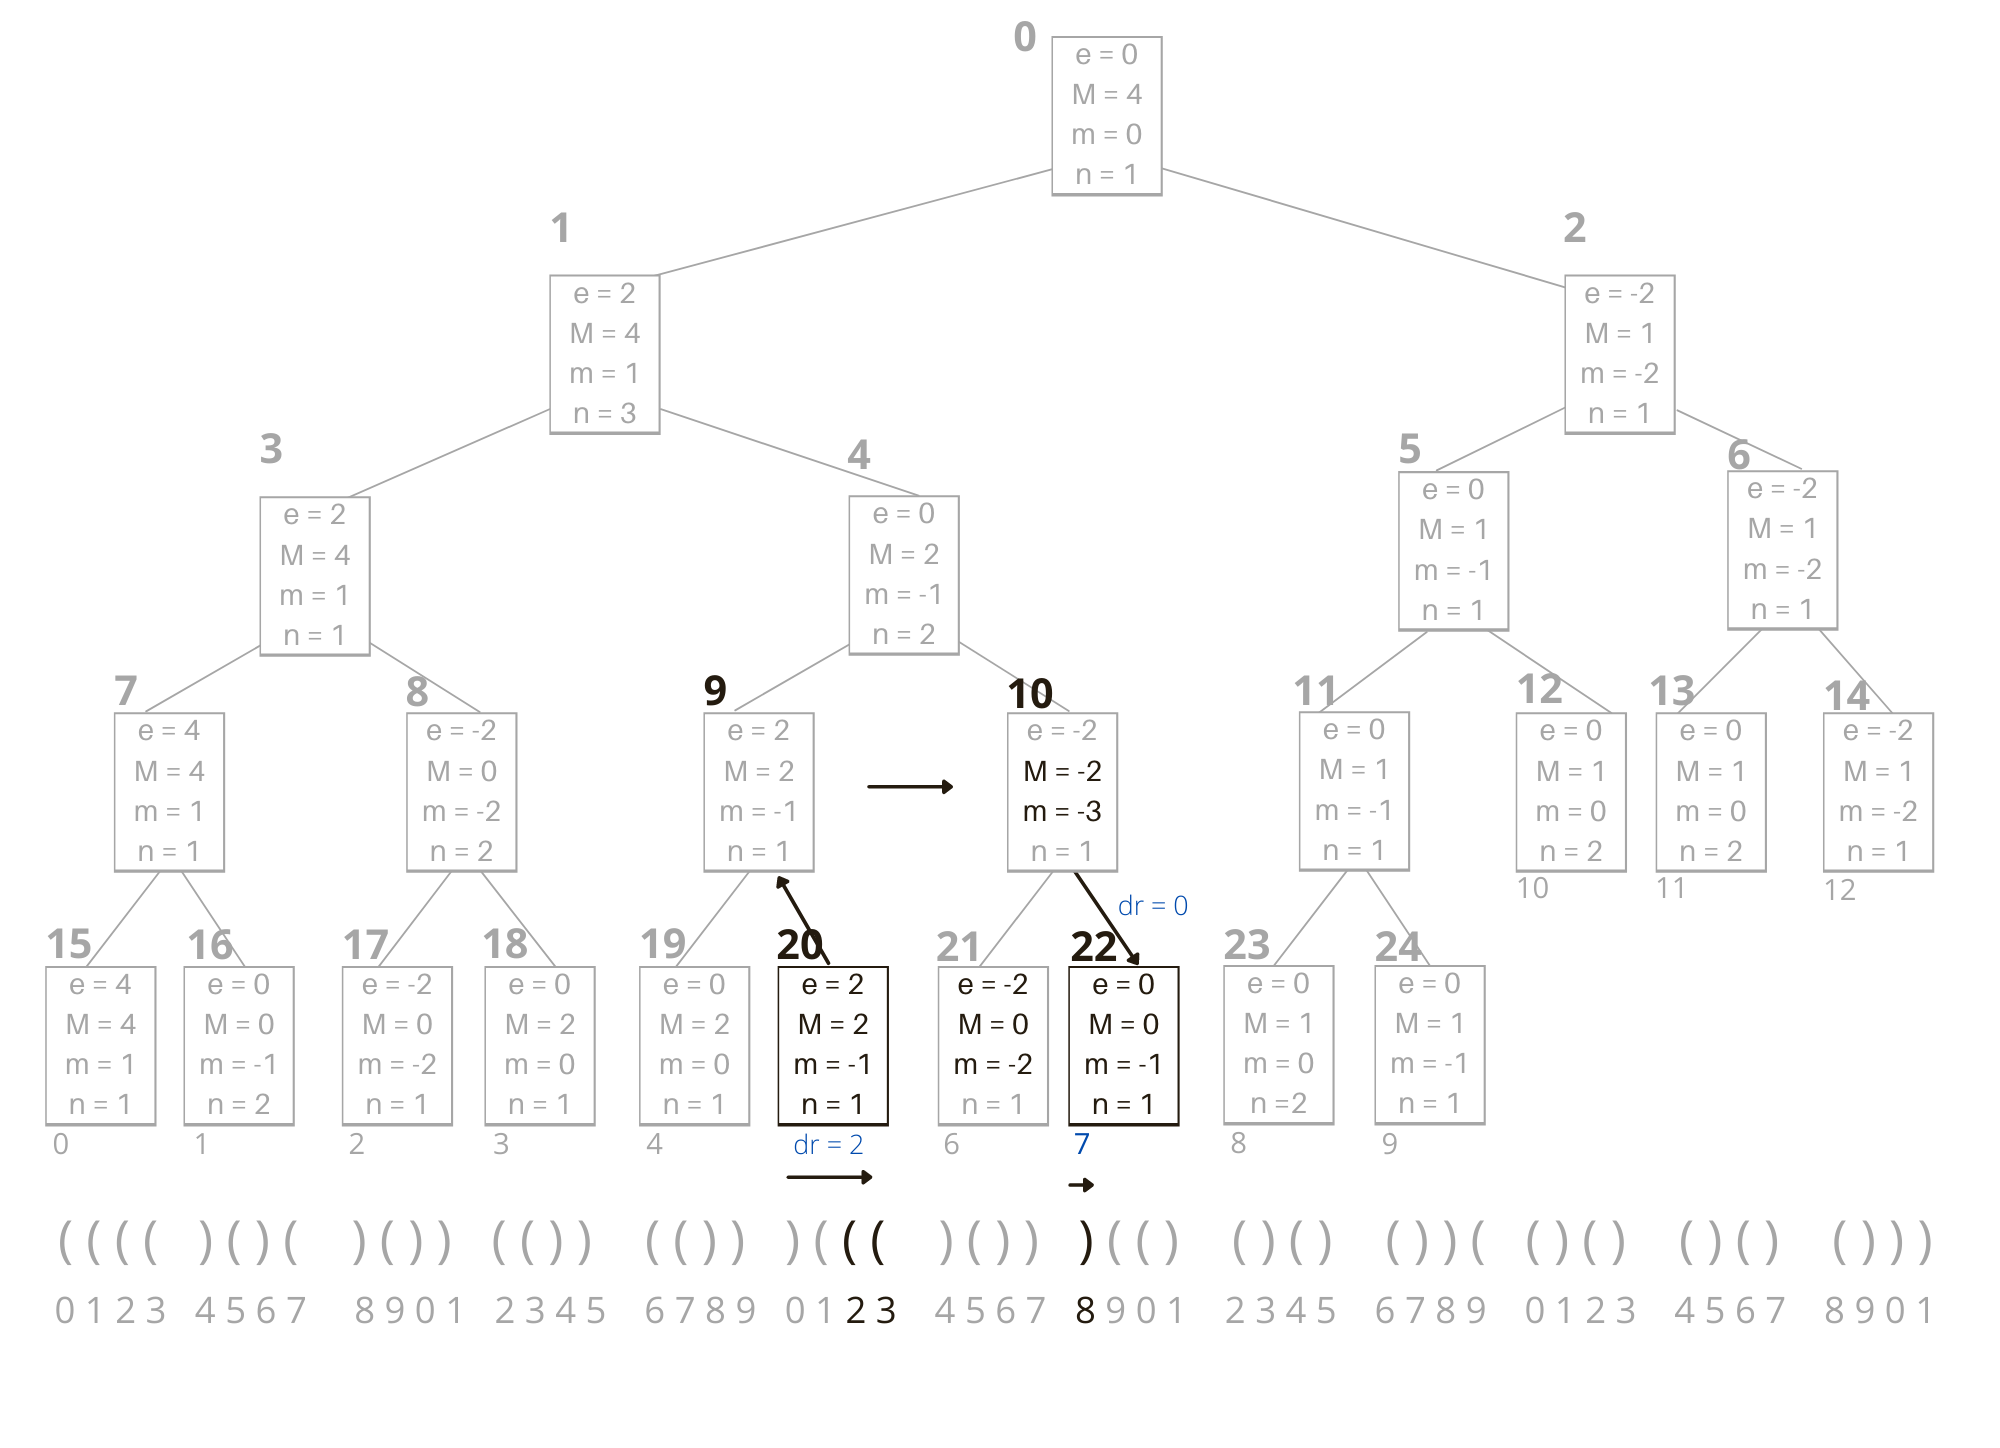
\includegraphics[width=\columnwidth]{images/rmm-tree-bin-fwdsearch.png}
             \label{fig:bin-fwdSearch}
        \end{figure}

        O processo é iniciado através da inspeção dos bits cobertos pelo nó $v=20$, os bits são inspecionados a partir da posição $i+1=22$, 
        até chegarmos ao
        fim do intervalo deste nó que é $j=23$, durante esse processo de inspeção simulamos a operação de $rank_($, 
        guardando em $dr$ os valores computados, ao fim do intervalo,
        temos que $dr=2$, 
        portanto precisamos aumentar o nosso intervalo de possibilidades, e como dito, 
        fazemos isso subindo na rmM-tree através dos seus nós, \citeauthor{book-compact-data-structures} traz um passo interessante que otimiza a busca na árvore, que consiste em 
        verificar o nó à direita do atual para verificar se a resposta se encontra nele, fazemo sesse processo olhando para os valores de excesso definidos no nó $20$,
         sem obter sucesso. Atualizanmos  então $v$ para $9$ (já sabemos que a resposta não está no nó $9$), 
         e verificamos se os campos do nó à direita ($10$) adicionados de $dr$, compreendem o excesso relativo buscado $d$, 
         ou seja $2 -3 \leq 1 \leq -2 +2$, essa asserção é válida, portanto, setamos $v$ como $10$. Iniciamos a descida na
         árvore, e como buscamos a posição $j$ mais à esquerda possível de $i$, verificamos primeiro se a resposta está contida no intervalo do filho esquerdo
        de nó $10$, a asserção não é validada, e portanto adicionamos à $dr$ o excesso local do nó $21$ ($dr + (-2)= 0$), 
        descemos então pelo filho direito de $v$, e nesse momento chegamos à
         um nó folha.
         
         Com esse processo reduzimos ao máximo o intervalo a ser inspecionado, neste momento inicia-se a varredura bit-a-bit no intervalo coberto pelo nó $22$. Nesse momento,
         temos que, $dr=0$ e $BP[28] = )$, logo $dr$ passe a valer $-1$, que é o exceso buscado inicialmente, e portanto a resposta para $fwdSearch(21,-1)$ é $j=28$.
    \end{example}
    
    \begin{algorithm}[h!]
        \Input{Índice $i$, a partir do qual a busca deve ser feita, excesso relativo $d$.}
        \Output{Posição $j$ onde ocorre $d$, ou $BP.size()$ caso a resposta não seja encontrada.}
        \vspace{.3cm}
        $dr \leftarrow 0$\\
        $j \leftarrow fwdBlock(i,d,\&dr)$ \tcp{Algoritmo~\ref{alg:fwdBlock}}
        
        \lIf{$dr = d $}{\Return{$j$}}
        $k \leftarrow \floor{(i+1)/b}$\\
        $v \leftarrow leafInTree(k)$\\

        \While{$(v+1)\&(v+2)$ \textbf{and} $dr + R[v+1].m \leq d \leq dr + R[v+1].M$}{
            \lIf{$v$  mod  $2$}{
                $dr \leftarrow dr + R[v+1].e$
            }
            $v \leftarrow \floor{(v-1)/2}$
        }

        \lIf{$(v+1)\&(v+2) = 0$}{\Return{$BP.size()$}}

        $v \leftarrow v +1 $\\

        \While{$v < numberLeaves -1 $}{
            \lIf{$dr + R[(2*v)+1].m \leq d \leq dr + R[(2*v)+1].M$}{
                $v \leftarrow (2*v) + 1 $
            }
            \Else{
                $dr \leftarrow dr + R[(2*v)+1].e$\\
                $v \leftarrow (2*v) +2$
            }
        }

        $k \leftarrow numLeaf(v)$\\
        $j \leftarrow fwdBlock((k*b)-1,d, \&dr)$\\
        \lIf{$dr = d$ }{\Return{$j$}}
        \lElse{\Return{$BP.size()$}}
        \caption{Busca por um excesso relativo $d$ através de $fwdSearch(i,d)$.}
        \label{alg:fwdSearch-bin}
    \end{algorithm}

    \begin{algorithm}[h!]
        \Input{Índice $i$ a partir do qual começamos a busca, excesso buscado $d$, excesso computado até o momento $\&dr$.}
        \Output{Posição $j$ onde ocorre a resposta, ou $BP.size()$ caso a resposta não exista.}
        \vspace{.3cm}
        $fb \leftarrow \ceil{(i+1)/w}$\\
        $lb \leftarrow \ceil{(i+2)/b}*(b/w)$\\
        \For{$j \leftarrow i+1$ \textbf{to} $(lb*w)-1$}{
            \lIf{$BP[j]=1$}{$dr \leftarrow dr + 1$}
            \lElse{$dr \leftarrow dr -1$}
            \lIf{$dr = d $}{\Return{$j$}}
        }

        \For{$p \leftarrow fb +1 $ \textbf{to} $lb$}{
            $x \leftarrow bitsRead((p-1)*w)$\\
            \lIf{$dr + C[x].m \leq d \leq dr + C[x].M$}{\textbf{break}}
            $dr \leftarrow dr + C[x].e$
        }

        \lIf{$p>lb$}{\Return{$lb*b$}}\tcp{dr não está no bloco subsequente}
        
        \For{$j \leftarrow (p-1)*w$ \textbf{to} $(p*w)-1$}{
            \lIf{$BP[j]=1$}{$dr \leftarrow dr + 1$}
            \lElse{$dr \leftarrow dr -1$}
            \lIf{$dr = d $}{\Return{$j$}}
        }
        \Return{$BP.size()$}
        \caption{Busca pelo excesso relativo $d$ em um nó folha, através de \textit{fwdBlock(i,d\&dr)}.}
        \label{alg:fwdBlock}
    \end{algorithm}

    \subsection{BwdSearch}\label{sc:bwdsearch}
    Essa operação é bastante similar à \textit{fwdSearch}, portanto não entraremos em tantos detalhes da mesma.
    Além disso mais à frente fornecemos um exemplo que esclarece o processo para esse tipo de busca.
    O ponto central de \textit{bwdSearch} é que, ao invés de realizarmos uma busca "à frente", como na operação anterior,
    realizamos uma busca "para trás", assim $bwdSearch$ busca por um índice $j < i$, mais à direita possível de $i$, tal que:
    $$bwdsearch(i,d) = max\{j < i | excess(j) = excess(i) - d\}$$

    Como explica \citeauthor{book-compact-data-structures}, a relação acima impacta na nossa busca através da rmM-tree devido aos dados
    armazenados nas nossas estruturas serem assimétricos, o autor faz então as seguintes considerações relacionadas ao processo de inspeção na rmM-tree,
    usando \textit{bwdSearch}:
    \begin{itemize}
        \item Buscamos por um excesso $j<i$, tal que:
         $$excess(j) - excess(i) = - excess(j+1,i) = d,$$ 
         isso faz com que o índice $i$ seja incluído na contagem;
        \item Queremos encontrar um índice $j$ tal que o excesso relativo computado,$dr$, de $i$ à $j$, seja igual ao excesso buscado, $d$.
         Mas como $j < i $ e portanto $dr = d = -excess(j+1,i)$,
        devemos adicionar $1$ unidade à $dr$ ao inspecionarmos um bit codificado como $0$, e diminuir $dr$ em $1$ unidade caso contrário;
        \item  Os registros de excesso são computados a partir de um processo de inspeção de bits da esquerda para a direita. \textit{bwdSearch}, realiza a pesquisa por excesso da direita para a esquerda, 
        isso implica que o excesso buscado $d$, é encontrado em um nó somente quando a asserção $dr - R[v].e + R[v].m \leq d \leq dr - R[v].e + R[v].M$ for válida.
    \end{itemize}
    O algoritmo~\ref*{alg:bwdSearch-bin} detalha mais sobre esse processo, este algoritmo invoca um método denominado \textit{bwdBlock}, este por usa vez é extremamente similar 
    ao algoritmo~\ref*{alg:fwdBlock} (a única ressalva é a questão de simetria discutida acima), portanto não fornecemos aqui \textit{bwdBlock}\footnote{Caso deseje ver como o mesmo é construído, ele 
    está disponível em nosso repositório}.
    \begin{example}
        Dado um nó em $BP$, codificado em $i=50$, encontrar o primeiro índice $j<i$,tal que $excess(j) - excess(i) = 0$


        Como no exemplo anterior, a figura \ref{fig:bin-bwdSearch}, destaca os bits e índices dos nós inspecionados para chegar a resposta esperada.
        \begin{figure}[h!]
           \centering
             \caption[bwdSearch(50,0).]{Simulação da operação $bwdSearch(50,0)$ em uma rmM-tree binária.}
             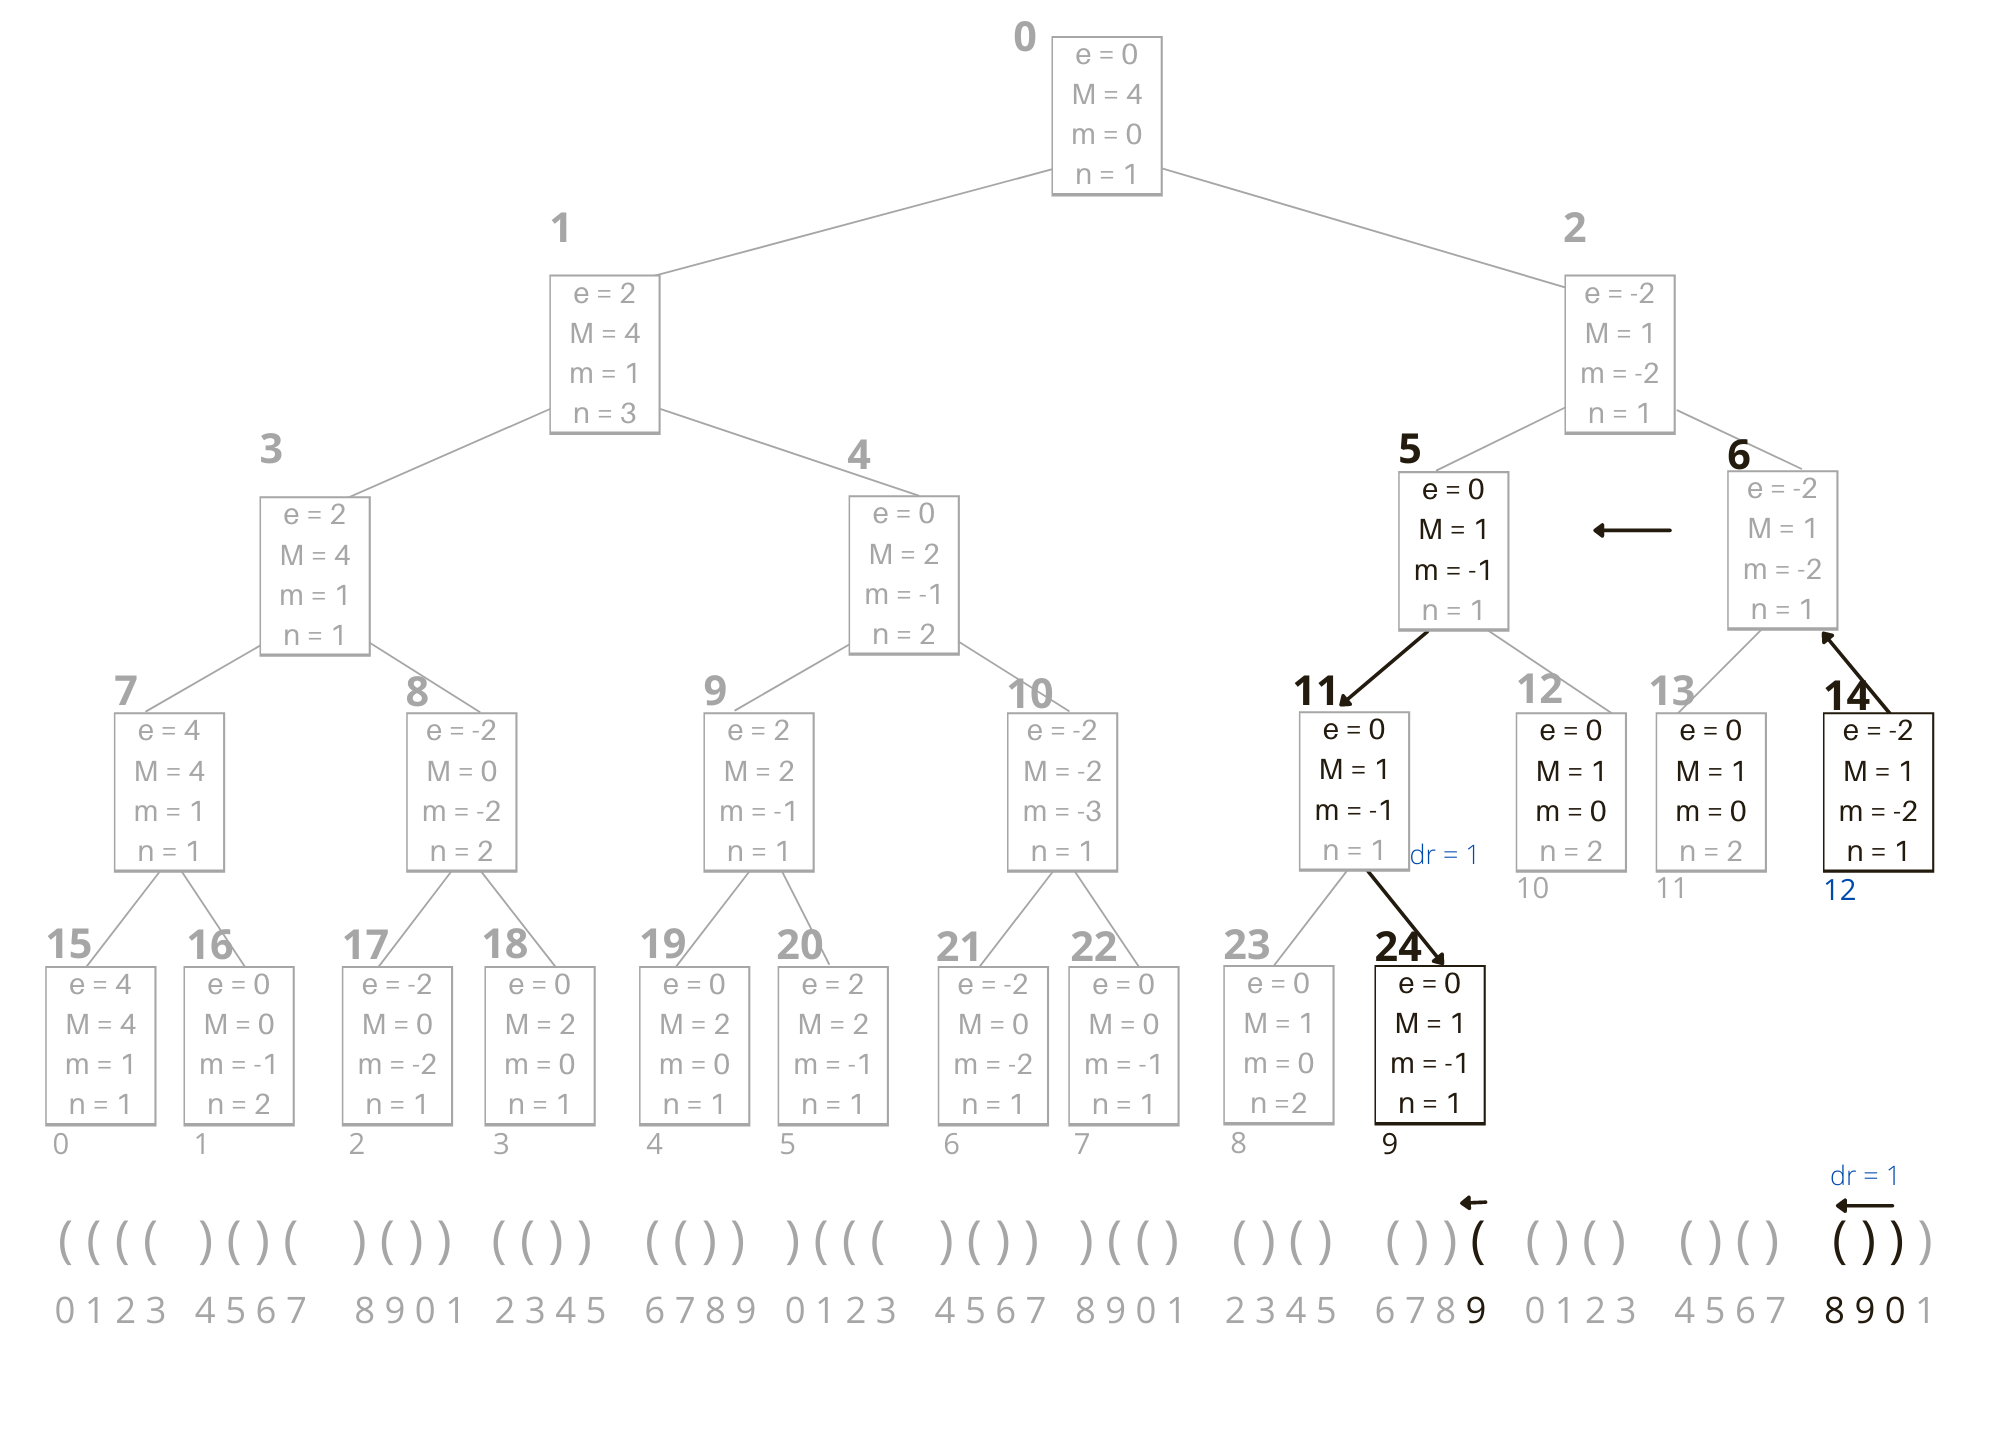
\includegraphics[width=\columnwidth]{images/rmm-tree-bin-bwdsearch.png}
             \label{fig:bin-bwdSearch}
        \end{figure}

        A nossa busca inicia a partir da inspeção dos bits compreendidos no intervalo da folha (nó $14$) que cobre o índice $i=50$, aos inspecionarmos os bits que
        vão de $i=50$ até $j=49$, temos que $dr=1$. Nesse momento $dr$ ainda é diferente do excesso buscado $d$, fazemos uma verificação no nó à esquerda 
        de $v$, e atestamos que o excesso procurado não está no intervalo do nó $13$. 
        Iniciamos a subida na árvore, atualizando $v$ para $6$, e antes de expandirmos o intervalo de busca navegando até o pai do nó $v$,
        analisamos o nó à esquerda de $v=6$, verificando se a asserção\footnote{$dr - R[v].e + R[v].m \leq d \leq dr - R[v].e + R[v].m$.} $ 1 -0 -1 \leq 0 \leq 1 -0 +1$
         é válida, obtemos uma resposta positiva, e por isso interropemos o processo de subida na rmM-tree. Começamos a descidana árvore
         a partir de $v=5$, verificamos se $d$ está contido no intervalo de excesso do filho direito de $v$ (lembrando, estamos buscando pelo $j$ mais à esquerda de $i$), 
         ou seja nó $12$, sem obter sucesso, prosseguimos a busca atualizando $v$ para o seu filho esquerdo.
         Verificamos agora se a asserção $dr - R[24].e + R[24].m \leq d \leq dr - R[24].e + R[24].m$ é válida para o filho direito do nó $11$,
         e temos que a mesma é válida, como chegamos à um nó folha, interrompemos a busca pelos nós da rmM-tree,
         e iniciamos uma busca mais detalhada em $BP[39,36]$ (de trás para frente), no índice $39$, $dr=d$ e portanto a busca através de $bwdSearch$ é encerrada retornando $j=39$.
    \end{example}

    \begin{algorithm}[h!]
        \Input{Índice $i$ a partir do qual a busca deve ser feita, excesso relativo $d$ desejado}
        \Output{Posição $j$ onde ocorre o $d$, ou $-1$ caso a resposta não seja encontrada}
        \vspace{.3cm}
        $dr \leftarrow 0$\\
        $j \leftarrow bwdBlock(i,d,\&dr)$ \tcp{Análogo ao algoritmo~\ref{alg:fwdBlock}}
        
        \lIf{$dr = d $}{\Return{$j$}}
        $k \leftarrow \floor{i/b}$\\
        $v \leftarrow leafInTree(k)$\\

        \While{$(v+1)\&v$ \textbf{and} $dr - R[v-1].e + R[v-1].m \leq d \leq dr - R[v].e + R[v-1].M$}{
            \lIf{$v$ mod $2 = 0$}{
                $dr \leftarrow dr - R[v-1].e$
            }
            $v \leftarrow \floor{(v-1)/2}$
        }

        \lIf{$(v+1)\&v = 0$}{\Return{$-1$}}

        $v \leftarrow v - 1 $\\

        \While{$v < numberLeaves -1 $}{
            \If{$dr - R[(2*v)+2].e + R[(2*v)+2].m \leq d \leq dr - R[(2*v)+2].e + R[(2*v)+2].M$}{
                $v \leftarrow (2*v) + 2$
            }
            \Else{
                $dr \leftarrow dr - R[(2*v)+2].e$\\
                $v \leftarrow (2*v) +1$
            }
        }

        $k \leftarrow numLeaf(v)$\\
        $j \leftarrow bwdBlock(((k+1)*b)-1,d, \&dr)$\\
        \lIf{$dr = d$ }{\Return{$j$}}
        \lElse{\Return{$-1$}}
        \caption{Busca por um excesso relativo $d$ através de $bwdSearch(i,d)$}
        \label{alg:bwdSearch-bin}
    \end{algorithm}

    \subsection{MinExcess}
    Esta é outra importante operação suportada pela rmM-tree. A partir dela podemos obter informações importantes sobre o nosso conjunto de dados, como o menor ancestral comum entre dois nós.
    
    
    O objetivo da \textit{minExcess}, é encontrar o excesso mínimo dentro de um intervalo $i, j$. Assim como para as outras operações, esta inicia-se a partir de uma inspeção bit-a-bit do intervalo que
    engloba o índice $i$, inspecionamos este intervalo fechado em $i$, até chegar ao fim do mesmo, ou até que cheguemos ao índice $j$.
    A cada cada bit inspecionado nesse processo, atualizamos o nosso excesso computado $d$, e verificamos se ele é o menor excesso computado até o momento (nesse caso atualizando o excesso mínimo computado).
    Terminando a inspeção deste bloco, caso $j$ não esteja contido nele, iniciamos o processo de subida na árvore (caso $j$ esteja contido, a busca é encerrada),
    nesse processo avaliamos se o excesso mínimo salvo em cada nó da rmM-tree é menor que o excesso mínimo computado até o momento,
    em caso afirmativo, atualizamos esse excesso mínimo, e  assim como nas outras operações, independente da resposta,
    atualizamos o excesso computado até o momento.
    Ressalta-se que o percurso em árvore para esta operação é idêntico ao percurso em árvore para \textit{fwdSearch},
    sendo interrompido, no momento em que estamos prestes a inspecionar um nó $v$, que seja ancestral do nó folha cujo intervalo engloba o índice $j$.
    Para tanto, precisamos de algumas evidências, trazidas por \citeauthor{book-compact-data-structures}, são elas:
    \begin{itemize}
        \item A profundidade de qualquer nó em $R[v]$ é dada por $\floor{\log v} +1$;
        \item O pai de um nó, é dado por $\floor{v/2}$, logo $u$ é ancestral de um nó $v$, se e somente se a asserção abaixo for válida,
        $$\floor{v/2^{\floor{log v} - \floor{log u}}} = v$$
        \item Conforme explica o autor, a asserção acima pode falhar quando o nó $u$ for um nó folha,
         e tiver uma profundidade maior que a do nó alvo
        (a folha que contém o índice $j$), de acordo com o autor isso pode ocorrer quando o número de folhas não for uma potência de $2$. 
        Para suprir esse problema devemos criar outro critério de continuação de subida na árvore, que é verificar se o índice do nó
        inspecionado é ou não, maior do que o índice do nó alvo, em caso afirmativo a busca prossegue com a subida na árvore.
    \end{itemize}


    Ao encontrarmos o ancestral do nó alvo, interrompemos o processo de subida na árvore, e começamos o processo de descida a partir deste ancestral,
     esse processo ocorre de modo similar aos outros,
    verificamos primeiro se o filho  esquerdo do nó visitado é ancestral do nó alvo. Em caso negativo usamos os valores de excesso deste nó 
    para verificar se existe um excesso mínimo menor que o computado até o momento,
    atualizamos esse valor conforme a resposta que obtivermos, e atualizamos o nosso nó corrente para o filho à direita deste nó. 
    Em caso positivo, atualizamos o nó corrente, para o seu filho esquerdo sem verificar os valores de excesso.
    Repetimos todo esse processo até que cheguemos a um nó folha, a partir daí fazemos uma inspeção bit-a-bit, até chegar na posição $j$, 
    e finalmente encerrando a busca tendo o menor excesso computado no intervalo $BP[i,j]$.


    O exemplo a seguir ilustra como o processo dessa operação é feito.
    \begin{example}
        Dado o intervalo $BP[18,39]$, retornar o menor excesso.

       \begin{figure}[!ht]
           \centering
             \caption[minExcess(18,39).]{Simulação da operação $minExcess(18,39)$ em uma rmM-tree binária.}
             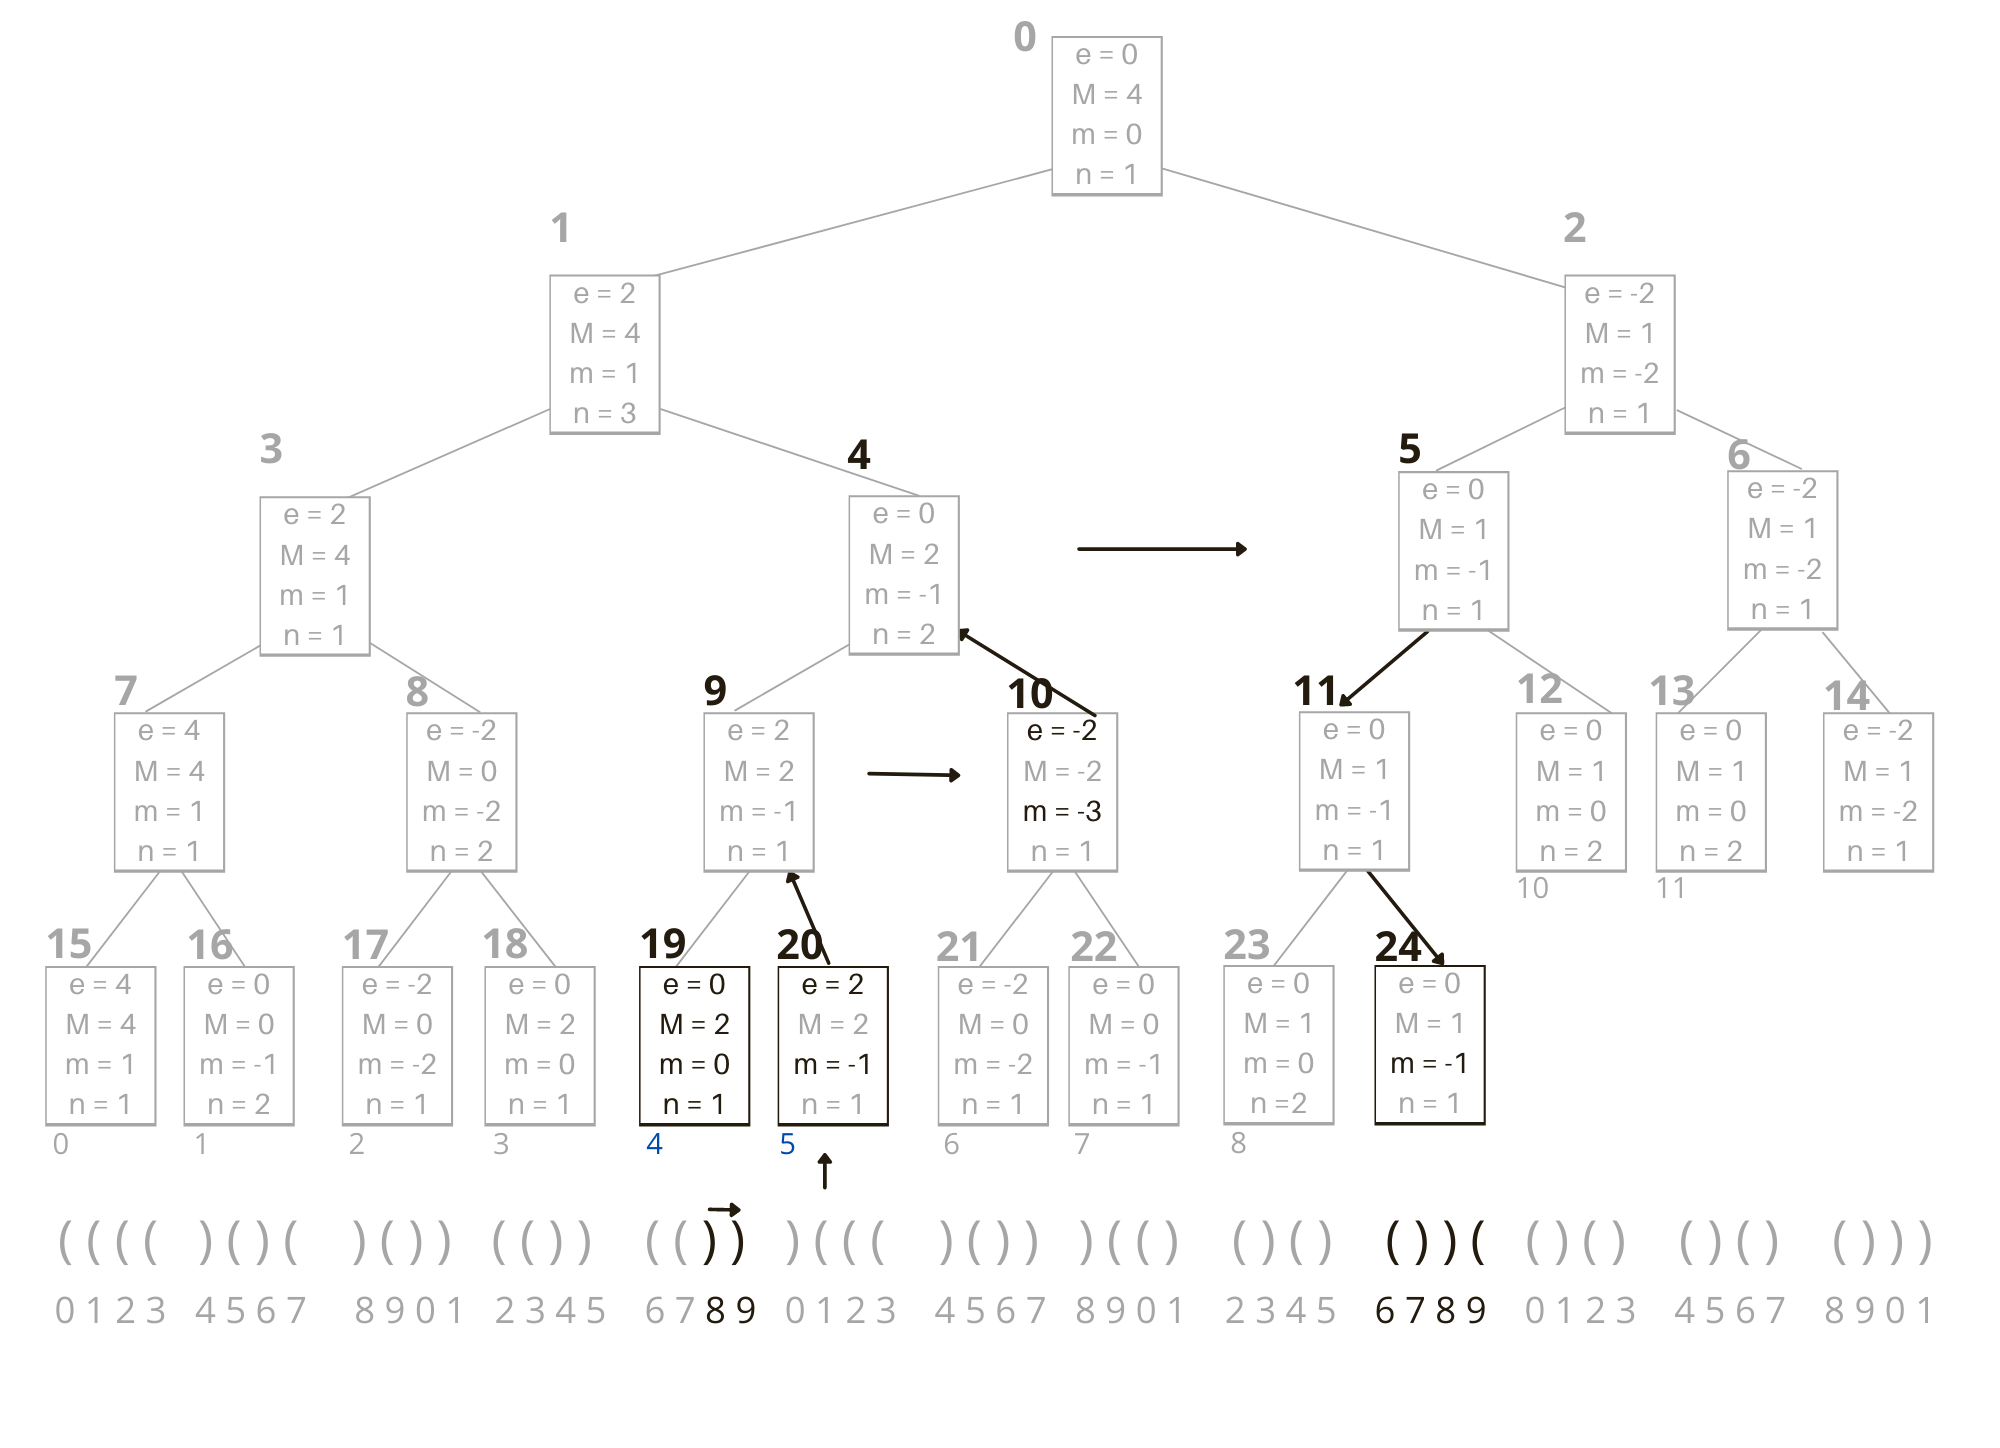
\includegraphics[width=\columnwidth]{images/rmm-tree-bin-minexcess.png}
             \label{fig:bin-minexcess}
        \end{figure}
        Varremos primeiramente o intervalo que vai de $i=18$ até $p=19$, nesse momento temos que o excesso mínimo ($m$) computado é $-2$, e o excesso local ($d$)
        é também $-2$. Como $j$ não está incluso no intervalo $18,19$, precisamos iniciar o processo de subida na árvore, antes disso identificamos o nó folha que cobre
        o intervalo de $j$, este nó é dado por $l=24$, verificamos, então se o excessmo mínimo no nó à direita de $v=19$, é menor que o excesso computado até o momento,
        como a asserção é válida $-2 -1 < -2$\footnote{$d + R[20].m < d]$}, atualizamos o valor de $m$ para $-3$, e o valor de $d$ para $0$.
        Subimos na árvore pelo nó $9$, e analisamos se o nó à direita, $v=10$,  é ancestral de $l$, e obtivemos uma negativa,
        atualizamos o valor de $d$ para $-2$, e subimos na árvore através do nó $4$. Novamente, verificamos se o nó à direita ($5$) do nó atual é ancestral do nó $l=24$, e nesse momento
        temos uma assertiva validada. Interrompemos e partir daqui iniciamos o processo de descida pela rmM-tree, a partir de $v=5$,
        como o filho esquerdo (nó $11$ ) de $v$, é ancestral do nó $24$, atualizamos $v$ para $11$. Em seguida, verificamos que o nó $23$ (filho esquerdo), 
        não é ancestral do nó $l=24$,  prosseguimos então para o filho direito, que é um nó folha e o próprio, nó $24$.
        Pecorremos os bits do intervalo coberto pelo nó $l$, até chegarmos à $j$, e, terminando a inspeção temos que o excesso mínimo em $BP[18,39]=-3$.
    \end{example}

        
        Uma outra variação dessa operação é a \textit{maxExcess}, o processo para responder está é completamente análogo, ao descrito acima, mudando apenas os registros da rmM-tree analisados, 
        ao invés de verificarmos o mínimo, verificamos o máximo.

    \subsection{MinCount e MinSelectExcess}
    Essas operações possuem bastate similaridade entre si, e também são análogas à \textit{minExcess}, portanto não entraremos em  detalhes sobre as duas, novamente, ambas 
    estão disponíveis em nosso repositório. 
    

    De modo geral, o objetivo da operação \textit{minCount} é computar o número de vezes que o excesso mínimo aparece no intervalo $BP[i,j]$, ao passo que a operação \textit{minSelectExcess}, 
    objetiva encontrar o índice dentro do intervalo $i,j$, onde ocorre a $t-$ésima ocorrência do excesso mínimo computado neste mesmo intervalo. 
    Observe que para ambas as operações, é necessário primeiro computar o excesso mínimo dentro do intervalo fornecido, para tanto, podemos fazer uma chamada a função \textit{minExcess}, 
    e então pecorrer a rmM-tree em busca da resposta esperada para cada operação. 
    
    Para operação \textit{minCount}, criamos um acumulador que é incrementado através do campo $n$, da rmM-tree, sempre que passarmos por um nó cujo o campo de excesso mínimo for igual ao excesso computado
    por \textit{minExcess}. 
    A operação \textit{minSelectExcess} segue pelo mesmo caminho, criamos um acumulador que recebe o valor $t$ passado para a função, e a diferença consiste no fato de que 
    ao encontrarmos um nó cujo o campo de excesso mínimo é igual ao valor computado por \textit{minExcess}, subtraímos do acumulador  o valor armazenado em $n$,
    a resposta nesse caso é encontrada quando o acumulador atingir a marca $0$. Para ambas as operações, o processo de subida e 
    descida na árvore se dá de igual modo ao mostrado em \textit{minExcess}.


    Essas são as únicas operações que usam o valor $n$ da rmM-tree, portanto não há necessidade de armazenar este, caso o objetivo da sua estrutura não englobe uma destas operações ou
    suas derivadas.

    \subsection{Derivadas}
    Esta seção demonstra como diversas operações sobre a rmM-tree podem ser escritas de modo eficiente a partir das operações descritas anteriormente.

    \begin{itemize}
        \item \textbf{rmq}: busca pela primeira posição onde ocorre o excesso mínimo computado dentro do intervalo  $BP[i,j]$. Ou seja:
            $$rmq(i,j) =\min \{ \argmin\{excess(p) | i \leq p \leq j\}\} $$
    
        Para à responder esta operação, podemos computar primeiro o exesso mínimo dentro do intervalo $i,j$, e em seguida realizar uma busca a partir de $i$.
        Temos assim:
        $$rmq(i,j) = fwdSearch(i-1,minExcess(i,j))$$
        Repare que o parâmetro do intervalo em \textit{fwdSearch} é subtraído em $1$, isso acontece porque o intervalo de busca define
        \textit{fwdSearch} é aberto, ou seja, não incluí o índice passado nas buscas, ao passo que o intervalo de \textit{rmq} é fechado, devendo incluir $i$ e 
        $j$ nas buscas. 
    
        \item \textbf{rMq}: similar a operação anterior, \textit{rMq}, busca a posição mais à esquerda de $i$ onde ocorre o excesso máximo computado em $i,j$. Ou seja:
        $$rMq(i,j) =\max\{ \argmax\{excess(p) | i \leq p \leq j\}\} $$   
        
        Assim:
            $$rMq(i,j) = fwdSearch(i-1, maxExcess(i,j))$$


        \item \textbf{findClose}: essa operação recebe como parâmetro um índice $i$, correspondente à um de abertura, e a partir da operação \textit{fwdSearch},
        busca o parênteses de fechamento correspondente. \textit{fwdSearch} irá fazer a varredura a partir de $i+1$ até encontrar o índice $j > i $, tal que 
        $excess(j) - excess(i+1) = -1 $.  Assim:
        $$findClose(i) = fwdSearch(i,-1)$$
            
        \item \textbf{findOpen}:  dado um índice, tal que $BP[i]=0$, \textit{findOpen}, faz uma busca por um $j < i $ tal que $excess(j) - excess(i) = 0$ e $excess(j)+1=1$. 
        Isso nos dá:
        $$findOpen(i) = bwdSearch(i,0)+1$$
        
        \item \textbf{enclose}: dado um índice $i$, que indica a codificação de um nó $x$, \textit{enclose} usará \textit{bwdSearch} para encontrar a posição $j<i$ mais à direita de $i$, 
        tal que $excess(j) - 2 = 1$. Ou seja:
        $$enclose(i) = bwdSearch(i,-2) + 1$$

        \item  \textbf{levelAncestor}: essa função buscará pelo nó $y$ que esteja $d$ níveis acima de um nó $x$, para tanto podemos usar \textit{bwdSearch},
        por questões de simetria, já discutidas anteriormente, devemos setar $d$ como negativo em \textit{bwdSearch}, e assim temos:
        $$levelAncestor(x,d) = bwdSearch(x,-d-1)+1$$
        
        \item \textbf{isAncestor}: essa função tem por objetivo verificar se um nó $x$ é ancestral de um nó $y$, para tanto basta verificar se $y$ está contido na hierarquia
        de $x$, podemos para tanto usar \textit{findClose}, do seguinte modo:
        $$ isAncestor(x,y) = (x < y  \mbox{ and }  y < findClose(x))$$
        
        \item \textbf{parent}: dado um índice $i$, correspondente ao bit que codifica um nó $x$, \textit{parent} busca através de \textit{enclose} o índice em $BP$ do nó que codifica
        o nó pai de $x$:
        $$parent(i) = enclose(i)$$
        
        \item \textbf{lca}: busca o menor ancestral comum entre dois nós, codificados nos índices $i$ e $j$. Existem 3 possibilidades de retorno para \textit{lca}, são eles:
        $$lca(i,j) =
               \begin{cases}
                     i,  \mbox{se } isancestor(i,j); \\
                    j, \mbox{se } isancestor(j,i); \\
                    parent(rmq(i ,j)+1)
               \end{cases}
        $$

        \item \textbf{deepestNode}: dado um nó em $BP$, \textit{deepestNode} retorna o filho com maior profundidade deste nó (localizado mais à esquerda possível).
        Sabemos que para calcular o maior excesso possível a partir de $i$ podemos usar a operação \textit{maxExcess}, como esse excesso deve estar limitado ao escopo do
        nó codificado em $i$, temos a seguinte relação:

        $$deepestNode(i) = rMq(i, findClose(i))$$

        A operação $rMq$ é usada aqui para invocar \textit{maxExcess} e em seguida retornar a posição exata onde ocorre o excesso computado.

        \item \textbf{degree}: esta operação contabiliza o número de filhos de um nó codificado em $i$, para simular ela, basta obter a quantidade de vezes que atingimos o excesso mínimo
        em $BP[i,findClose(i)]$, excluindo os limites que definem este nó, ou seja:
        $$degree(i) = minCount(i+1, findClose(i)-1)$$
        
        \item \textbf{childRank}: dado um índice $i$, \textit{childRank}, contabiliza o número de irmãos que o nó codificado em $i$ possuí à sua esquerda, tendo as operações definidas anteriormente,
        podemos responder à esta operação do seguinte modo:
        $$
               childRank(i) = minCount(parent(i)+1, i) +1
        $$
        
        \item \textbf{nextSibling}: dado um nó codificado em $i$, \textit{nextSibling} busca pelo nó codificado em $j$, tal que $j>i$.
        $$nextSibling(i) = findClose(i) +1$$
        
        \item \textbf{prevSibling}: análaga a \textit{nextSibling}, esta operação busca pelo irmão imediatamente à esquerda do nó codificado por $i$ em BP. Ou seja:
        $$prevSibling(i) = findOpen(i-1)$$
        
        \item \textbf{child}: dado um índice $i$ que codifica um nó, \textit{child} calcula a posição em $BP$ onde ocorre a codificação do $t-$ésimo filho de $i$. 
        Ou seja, ela calcula o índice onde ocorre pela $t-$ésima vez o excesso mínimo dentro do intervalo do nó $i$, desse modo, podemos escrever
        \textit{child} em função de \textit{findClose} e \text{minSelectExcess}:
        $$p = findClose(i)$$
        $$child(i) = minSelectExcess(i+1,p-1,t-1) + 1 $$

        \item \textbf{lastChild}: busca pelo último filho de um nó codificado em um índice $i$:
        $$lastChild(i) = findOpen(findClose(i)-1)$$
        
        \item  \textbf{subtreeSize}: calcula o tamanho da subárvore enraízada no nó $i$, para tanto, basta realizar uma contagem dos nós codificados no intervalo do 
        nó $i$, ou seja:
        $$subtreeSize(i)= \floor{(findclose(i) - i + 1)/2}$$
        
        \item \textbf{levelNext}: busca o nó mais a direita do nó codificado por $i$, em seu mesmo nível:
        $$levelNext(i) = fwdSearch(findClose(i),1)$$
        
        \item \textbf{levelPrev}: análaga a \textit{levelNext}, esta função busca pelo primeiro nó a esquerda do nó codificado em $i$, que possuí a mesma profundidade deste. 
        Como estamos falando de uma busca à esquerda de um índice, usamos \textit{bwdSearch} para realizar está operação:
        $$levelPrev(i) = findOpen(bwdSearch(i,0)+1)$$
        
        \item \textbf{levelLeftMost}: busca pelo nó mais à esquerda da raíz, com profundidade $d$, assim:
        $$levelLeftMost(d) = fwdSearch(0,d-1)$$
        
        \item \textbf{levelRightMost}: usando como referência a raíz, busca pelo nó mais à direita, cuja profundidade é igual  à $d$:
        $$levelRightMost = findOpen(bwdSearch(BP.size()-1,d)+1)$$
    \end{itemize}
    
    Algumas das operações a seguir, além das nossas primitivas, usam em seu escopo as operações suportadas pela estrutura de vetores de bits 
    (algumas, como o caso de \textit{depth} usam apenas estás últimas). Isso nos
    mostra também a importância do cuidado ao escolhermos uma estrutura de suporte apropriada afim de acelerar nossas operações:
        \begin{itemize}
            \item \textbf{firstChild}: retorna o primeiro filho do nó codificado por $i$, logo:
            $$firstChild(i) = i +1$$
            \item \textbf{isLeaf}: dado um nó codficiado em $i$, verifica se este é um nó folha ou não, essa é uma das operações mais simples da nossa estrutura e necessista apenas de 2 comparações, veja abaixo:
            $$isLeaf(i) = (BP[i] == 1 \mbox{ and } BP[i+1]==0)$$
            \item \textbf{depth}: computa a profundidade de um nó codficado por $i$, para tanto basta verificar o exesso em $BP[0,i]$, ou seja:
            $$depth(i) = excess(i)$$
            \item \textbf{leafRank}: contabiliza a quantidade de folhas existente em um intervalo que vai de $0$ à $i$. Em nossa implementação, usamos a operação \textit{rank},
            suportada pela estrutura de vetores de bits. Assim, basta buscar a quantidade de ocorrêncas de bits $1$ seguidos por bit $0's$.
            $$leafRank(i) = rank_{10}(i)$$
            \item \textbf{leafSelect}: esta operação nos permite buscar pela $i-$ésima folha em $BP$, para essa operação buscamos pela $i-$ésima ocorrência do padrão $10$:
            $$leafSelect(i) = select_{10}(i)$$
            \item \textbf{leftMostLeaf}: retorna o índice da folha localizada mais à esquerda do nó codificado em $i$.
            $$leftMostLeaf(i) = leafSelect(leafRank(x-1)+1)$$
            \item  \textbf{rightMostLeaf}: busca a folha mais à direita do nó codificado em $i$:
            $$rightMostLeaf(i) = leafSelect(leafRank(findClose(i)))$$
            \item \textbf{preRank}: calcula a quantidade de ancestrais de um nó codificado em $i$.
            $$preRank(i) = rank_1(i)$$
            \item \textbf{postRank}: calcula a quantidade de ancestrais do nó $i$  somados aos seux $x$ filhos.
            $$postRank(i) = rank_0(findClose(i))$$
            \item \textbf{preSelect}: retorna a posição do $i-$ésimo nó, usando um percurso pré-ordem:
            $$preSelect(i) = select_1(i)$$
            \item \textbf{postSelect}: retorna a posição do $i-$ésimo nó, usando um percuso pós-ordem, nesse caso podemos usar \textit{findOpen} que é derivada da nossa primitiva \textit{bwdSearch}:
            $$postSelect(i) = findOpen(select_0(i))$$
        \end{itemize} 

%a tabela~\ref{tbl:classicOperations-rmm-tree}  mostra as operações suportadas por essa estrutura.
\begin{table}[h!]
	\centering
	\caption[Operações sobre a RMM-tree clássica]{Operações suportadas pela rmM-tree bináriaW}
	\label{tbl:classicOperations-rmm-tree}
	\rowcolors{2}{lightgray!30}{white}
	\resizebox{\columnwidth}{!}{
	\begin{tabular}{ll}
	\toprule
	\textbf{Operação} & \textbf{Retorno} \\
	\toprule
    
	fwdSearch(i,d)  & Índice $j$, tal que $excess(j) = excess(i) + d$\\
	bwdSearch(i,d)  & Índice $j$, tal que $excess(j+1,i) = -d$\\
	minExcess(i,j) / maxExcess(i,j)  & Excesso mínimo/máximo em $i,j$\\
	minCount(i,j)  & Número de vezes que o excesso mínimo aparece em $i,j$\\
	minSelectExcess(i,j,t)  & Índice da $t-$ésima ocorrência do excesso mínimo em um intervalo\\
	enclose(i) & Posição do parênteses de abertura que envolve  $BV[i]$  \\
	rmq(i,j) / rMq(i,j) & $p>=i$ mais à esquerda de $i$, onde ocorre o excesso mínimo/máximo do intervalo dado \\
	rank$_1$(i) / rank$_0$(i) & Número de parênteses abrindo/fechando em $BV[0,i]$ \\
    select$_1$(i) / select$_0$(i) & Posição do i-ésimo parênteses de abertura/fechamento\\
    preRank(i)/postRank(i) & rank de $i$ calculado a partir de um percurso \textit{preorder \mbox{ ou } postorder} \\
    preSelect(i)/postSelect(i) & retorna o nó com \textit{preorder/postorder} $i$\\
    isLeaf(i) & Verifica se $BV[i]$ codifica uma folha \\
    isAncestor(i,j) & Verifica se o nó codificado em $i$ é ancestral de $j$ \\
    depth(i) & Profundidade do nó $i$ \\
    parent(i) & Obtém o pai do nó $i$ \\
    firstChild(i) / lastChild(i) & Retorna o primeiro/último filho do nó codficiado em $BV[i]$ \\
    child(i,t)&$t-$ésimo filho do nó codificado em $i$\\
    nextSibling(i) / prevSibling(i) & Primeiro irmão à direita/esquerda de $i$ \\
    subtreeSize(i) & Número de nós enraízados na subárvore de $i$ \\
    levelAncestor(i,d) & Ancestral $j$ de $i$ tal que $depth(j) = depth(i) - d$\\
    levelNext(i) / levelPrev(i) & Nó à direita/esquerda de $i$ com a mesma profundidade de $i$.\\
    levelLeftMost(d) / levelRightMost(d) &Nó mais à esquerda/direita, com profundidade d.\\
    lca(i,j)&Menor ancestral comum dos nós codificados em $i$ e $j$\\
    deepestNode(i)&Nó mais profundo de $i$ (mais à direita possível)\\
    degree(i)&Número de filhos do nó $i$ \\
    childRank(i)&Número de irmãos à esquerda do nó codificado em $i$\\
    leafRank(i)& Número de folhas à esquerda da folha codificada em $i$ \\
    leafSelect(i)& $i-$ésima folha em $BV[0,size-1]$ \\
    leftMostLeaf(i)& folha codificada em $j$, mais à direita de $i$, tal que $j<i$\\
    rightMostLeaf(i)& folha codificada em $j$, mais à direita possível, tal que $j \leq i$\\
	\bottomrule
	\end{tabular}
	}
\end{table}



\section{rmM-tree k-ária}
Apesar da range min-Max tree possuir um desempenho satisfatório, obedecendo ao limite de espaço definido pela teoria informação e oferecendo suporte à diversas operações em tempo eficiente,
quando se trabalha com grandes conjuntos de dados a mesma pode realizar muitas transferências entre cache e memória RAM.
Isso se deve ao fato de que a rmM-tree é uma árvore construída no formato de árvore binária, o que implica em um fator de ramificação baixo, acarretando em uma perda na localidade espacial durante o processo de navegação na árvore.

Como vimos em outros trabalhos, aumentando o número de ramificações de uma árvore, podemos sanar os problemas acima citados.
Nosso objetivo portanto com este trabalho é propor um tipo de rmM-tree com um número maior de ramificações, a proposta para essa estrutura será melhor detalhada no capítulo a seguir.
%\citet{paper-making-btree-cache} usam o mesmo príncipio do alto fator de ramificação das árvores B e seu melhor aproveitamento de cache em relação às árvores binárias para construir uma variação de Árvores Sensíveis a Cache (CSS-Tree). Os autores usaram uma variação das árvores B+ que armazena os seus nós de forma contígua (possiblitando assim o armazenamento apenas do endereço do primeiro filho em um nó), maximizando assim  o espaço de armazenamento dos índices, e em decorrência disso diminuindo ainda mais o fator de ramificação. Os resultados experimentais deste trabalho, mostraram 

